\documentclass[	DIV=calc,paper=a4,fontsize=11pt]{scrartcl}	 	% KOMA-article class
\usepackage{lipsum}		
\usepackage[margin=1in]{geometry}								% Package to create dummy text
\usepackage[english]{babel}										% English language/hyphenation
\usepackage[protrusion=true,expansion=true]{microtype}			% Better typography
\usepackage{amsmath,amsfonts,amsthm,amssymb}					% Math packages
\usepackage[pdftex]{graphicx}									% Enable pdflatex
\usepackage[svgnames]{xcolor}									% Enabling colors by their 'svgnames'
\usepackage[hang, small,labelfont=bf,up,textfont=it,up]{caption}	% Custom captions under/above floats
\usepackage{epstopdf}												% Converts .eps to .pdf
\usepackage{subfig}													% Subfigures
\usepackage{tikz}
\usetikzlibrary{shapes,snakes}
\usepackage{booktabs}												% Nicer tables
\usepackage{fix-cm}		
\usepackage[bookmarks=true]{hyperref}

\newtheorem{thm}{Theorem}[section]
\newtheorem{lem}[thm]{Lemma}
\newtheorem{prop}[thm]{Proposition}
\newtheorem{cor}[thm]{Corollary}
\newtheorem{conj}[thm]{Conjecture}

\theoremstyle{definition}
\newtheorem{defn}[thm]{Definition}
\newtheorem{defns}[thm]{Definitions}
\newtheorem{con}[thm]{Construction}
\newtheorem{exmp}[thm]{Example}
\newtheorem{notn}[thm]{Notation}
\newtheorem{notns}[thm]{Notations}
\newtheorem{addm}[thm]{Addendum}
\newtheorem{exer}[thm]{Exercise}
\newtheorem{rem}[thm]{Remark}
\theoremstyle{plain}


\theoremstyle{remark}
\newtheorem{rems}[thm]{Remarks}
\newtheorem{warn}[thm]{Warning}
\newtheorem{sch}[thm]{Scholium}
\DeclareMathOperator{\id}{id}

\newcommand{\bd}[1]{\mathbf{#1}}  % for bolding symbols
\newcommand{\RR}{\mathbb{R}}      % for Real numbers
\newcommand{\ZZ}{\mathbb{Z}}      % for Integers
\newcommand{\col}[1]{\left[\begin{matrix} #1 \end{matrix} \right]}
\newcommand{\comb}[2]{\binom{#1^2 + #2^2}{#1+#2}}
%%% Custom sectioning (sectsty package)
\usepackage{sectsty}												% Custom sectioning (see below)
\allsectionsfont{%													% Change font of al section commands
	\usefont{OT1}{phv}{b}{n}%										% bch-b-n: CharterBT-Bold font
	}

\sectionfont{%														% Change font of \section command
	\usefont{OT1}{phv}{b}{n}%										% bch-b-n: CharterBT-Bold font
	}



%%% Headers and footers
\usepackage{fancyhdr}												% Needed to define custom headers/footers
	\pagestyle{fancy}												% Enabling the custom headers/footers
\usepackage{lastpage}	

% Header (empty)
\lhead{}
\chead{}
\rhead{}
% Footer (you may change this to your own needs)
\lfoot{\footnotesize \texttt{www.albohessab.weebly.com} \textbullet}
\cfoot{(DRAFT-VERSION)}
\rfoot{\footnotesize page \thepage\ of \pageref{LastPage}}	% "Page 1 of 2"
\renewcommand{\headrulewidth}{0.0pt}
\renewcommand{\footrulewidth}{0.4pt}


\usepackage{tcolorbox}
%%% Creating an initial of the very first character of the content
\usepackage{lettrine}
\newcommand{\initial}[1]{%
     \lettrine[lines=3,lhang=0.3,nindent=0em]{
     				\color{DarkGoldenrod}
     				{\textsf{#1}}}{}}

\makeatletter
\def\@xfootnote[#1]{%
  \protected@xdef\@thefnmark{#1}%
  \@footnotemark\@footnotetext}

%%% Title, author and date metadata
\usepackage{titling}															% For custom titles

\newcommand{\HorRule}{\color{DarkGoldenrod}%			% Creating a horizontal rule
									  	\rule{\linewidth}{1pt}%
										}

\pretitle{\vspace{-30pt} \begin{flushleft} \HorRule
				\fontsize{25}{25} \usefont{OT1}{phv}{b}{n} \color{DarkRed} \selectfont
				}
\title{$\mathbb{MY\ REAL\ ANALYSIS \ NOTE}$}					% Title of your article goes here
\posttitle{\par\end{flushleft}\vskip 0.5em}

\preauthor{\begin{flushleft}
					\large \lineskip 0.5em \usefont{OT1}{phv}{b}{sl} \color{DarkRed}}
\author{Miliyon T.,}											% Author name goes here
\postauthor{\footnotesize \usefont{OT1}{phv}{m}{sl} \color{Black}
		\\ \textbf{A}dama \textbf{S}cience and \textbf{T}echnology \textbf{U}niversity % Institution of author
					\par\end{flushleft}\HorRule}

\date{\today}											% No date



%%% Begin document
\begin{document}
\clearpage
\maketitle
\thispagestyle{empty}
\initial{R}\textbf{eal analysis is a branch of mathematical analysis dealing with the real numbers and real-valued functions of a real variable. In particular, it deals with the analytic properties of real functions and sequences, including convergence and limits of sequences of real numbers, the calculus of the real numbers, and continuity, smoothness and related properties of real-valued functions.}

\medskip

\noindent \textbf{Real Analysis is a very straightforward subject, in that it is simply a nearly linear development of mathematical ideas we have come across throughout our story of mathematics. However, instead of relying on sometimes uncertain intuition (which we have all felt when we were solving a problem we did not understand), we will anchor it to a rigorous set of mathematical theorems.}

\medskip
\noindent\textbf{\footnote[*]{\textbf{Typeset in \LaTeX}}This note covers the material in Math $661\ \&$ Math $666$.}
\vfil

\begin{center}
\copyright ~Miliyon Tilahun
\end{center}
\newpage
\tableofcontents
\newpage
\thispagestyle{fancy} 			% Enabling the custom headers/footers for the first page
% The first character should be within \initial{}


\section{Finite, infinite and countable sets}

\begin{quote}
"The usefulness of a pot comes from its emptiness."
\end{quote}

\subsection{Definition}

\begin{defn}[\textbf{\color{blue}{Set}}]
A collection of objects called \textit{members} or \textit{elements} of the set.
\end{defn}

\begin{defn}[\textbf{\color{blue}{Relation}}]
A well defined collection of objects called \textit{members} or \textit{elements} of the set.
\end{defn}

\begin{defn}[\textbf{\color{blue}{Function}}]
Given two sets $A$ and $B$, by a mapping or function from $A$ into $B$ we mean a correspondence that assigns to each member of $A$ a member of $B$.
\end{defn}

\begin{defn}[\textbf{\color{blue}{Equivalence relation}}]
A relation $R$ on a set $A$ is an equivalence relation if it satisfies
\begin{description}
  \item[(i)] Reflexive: $(a,a)\in R,\ \forall a\in A$.
  \item[(ii)] Symmetric: $(a,b)\in R\Rightarrow (b,a)\in R,\ \forall a,b\in A$.
  \item[(iii)] Transitive: $(a,b),(b,c)\in R\Rightarrow (a,c)\in R,\ \forall a,b,c\in A$.
\end{description}
\end{defn}

\begin{defn}[\textbf{\color{blue}{Finite}}]

\end{defn}
\subsection{Facts}

\begin{thm}
Every infinite subset of a countable set $A$ is countable.
\end{thm}

\begin{proof}
Exercise
\end{proof}


\begin{thm}
The union of a countable set is countable.
\end{thm}

\begin{proof}
Exercise
\end{proof}

\newpage
\begin{thm}
The set of rational numbers are countable.
\end{thm}

\begin{proof}
Write the rational number as $m/n$, where $m$ and $n$ are integers that are relatively prime. Let $m = p_1^{e_1}\cdot p_2^{e_2}\cdots p_k^{e_k}$ and $n = q_l^{f_1} \cdot q_2^{f_2}\cdots q_t^{f_t}$ be the prime-number decompositions of $m$ and $n$. Then the desired counting function for the rational numbers is $f(1) = 1$
and
\[f\biggl(\frac{m}{n}\biggl)=p_1^{2e_1}\cdot p_2^{2e_2}\cdots p_k^{2e_k}\cdot q_l^{2f_1-1} \cdot q_2^{2f_2-1}\cdots q_t^{2f_t-1}\]

This function is uniquely invertible. For example, the rational number $\frac{2}{3}$ is the twelfth number on the list; and the eighteenth number on the list is $\frac{3}{2}$.

\medskip

Consider the following figure
\begin{figure}[hbt!]
\centering
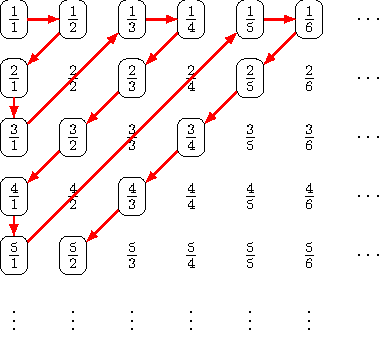
\includegraphics[width=.4\textwidth]{rational}
\caption{Cantor's diagonal method}
\end{figure}

This is the best way of exhausting the rational numbers.
\end{proof}

\newpage
\subsection{Exercise}
\begin{exer}\label{001}
$\mathbb{R}$ the set of real numbers is uncountable.
\end{exer}

\begin{exer}\label{002}
The set of all polynomial
  \[ p(x)=a_0+a_1x+a_2x^2+\cdots+a_nx^n\]
with $a_i\in\mathbb{Z}, \forall i\in\{1,2,\ldots,n\}$ is countable.
\end{exer}

\begin{exer}\label{003}
The set of algebraic number is denumerable.
\end{exer}

\begin{exer}\label{004}
$S$ be a set of all sequences of $0$'s and $1$'s i.e. $S=\{(a_1,a_2,a_3,\ldots)|a_n=0\text{ or } 1\}$. Show that $S$ is uncountable.
\end{exer}

\newpage
\subsection*{Solution}
\begin{proof}[Solution (\ref{001})]\footnote{Cantor diagonal proof}
First, we show the subset $(0,1)$ of the real numbers is uncountable, then it follows $\Bbb R$ is uncountable.

  The set of real numbers in $(0,1)$ can be written as decimals of the form
  $$
  \begin{array}{rlllll}
  0\;.&d_{11}&d_{12}&d_{13}&d_{14}&\ldots\\
  0\;.&d_{21}&d_{22}&d_{23}&d_{24}&\ldots\\
  0\;.&d_{31}&d_{32}&d_{33}&d_{34}&\ldots\\
  0\;.&d_{41}&d_{42}&d_{43}&d_{44}&\ldots\\
  \vdots\; & \;\vdots&\;\vdots&\;\vdots\;&\vdots&\ddots
  \end{array}
  $$
  where $d_{ij}$'s are all digit from the set $\{0,1,2,\ldots,9\}$.

  Assume, there exist a one-to-one correspondence between the decimals in $(0,1)$ and $\Bbb N$.

  \[ \Bbb N \left\{\begin{array}{rllllll}
  1 & \leftrightarrow \quad0\;.&d_{11}&d_{12}&d_{13}&d_{14}&\ldots\\
  2 & \leftrightarrow \quad0\;.&d_{21}&d_{22}&d_{23}&d_{24}&\ldots\\
  3 & \leftrightarrow \quad0\;.&d_{31}&d_{32}&d_{33}&d_{34}&\ldots\\
  \vdots\; & \;\vdots&\;\vdots&\;\vdots\;&\vdots&\vdots \\
  n & \leftrightarrow \quad0\;.&d_{n1}&d_{n2}&d_{n3}&d_{n4}&\ldots\\
  \vdots\; & \;\vdots&\;\vdots&\;\vdots\;&\vdots&\vdots&\ddots
  \end{array}\right\} (0,1)
\]
We will now construct a decimal in $(0,1)$, which is missed by this correspondence.\\
Construct $x=0.c_1c_2c_3\ldots$
\begin{align*}
\text{where  } c_1&\neq d_{11},0,9.\\
               c_2&\neq d_{22},0,9.\\
               c_3&\neq d_{33},0,9.\\
                  &\vdots
\end{align*}
We forbid $0$ and $9$ so that $x\neq 0.000\ldots=0$, $x\neq0.999\ldots=1$, and to have a unique representation.\\
By construction this number $x$ is in $(0,1)$ and differ from the $n^{th}$ decimal number in the sequence in the $n^{\scriptscriptstyle \text{th}}$ decimal digit.
So, $x$ is missed by the supposed correspondence. Hence, our assumption that there exist a correspondence between $(0,1)$ and $\Bbb N$ is incorrect. Thus, the set $(0,1)$ is uncountable.\\
Therefore, $\Bbb R$ is uncountable.
\end{proof}
\begin{proof}[Solution (\ref{002})]
For each pair of integers $(n,m)\in \Bbb N\times \Bbb N$, let $P_{nm}$ denote the set of polynomials of degree $m$ in which
  \[|a_0|+|a_1|+\cdots+|a_m|=n\]
  $P_{nm}$ is finite for each $n,m\in \Bbb N$. Hence
  \[P=\bigcup\{P_{nm}:(n,m)\in \Bbb N\times \Bbb N\}\]
  is countable since it is a countable union of countable sets.
\end{proof}
\begin{proof}[Solution (\ref{003})]
Let $P_n[x]$ be the set of polynomial functions with rational coefficients. Then there is a bijection from $P_n[x]$ into $\Bbb Q^n$. Since $\Bbb Q$ is countable, there exists a bijection $f : \Bbb Q\to \Bbb N$. Hence the map $F : \Bbb Q^n\to \Bbb N^n$ defined by $F (r_1,\ldots, r_n) = (f(r_1),\ldots, f(r_n))$ is a bijection. Since $\Bbb N^n$ is countable, we conclude that $\Bbb Q^n$ is countable and consequently $P_n[x]$ is countable. The set
      $$R_n = \bigcup_{P\in P_n[x]}\{x \in \Bbb R; P (x) = 0\}$$
is countable since it is a countable union of finite sets. Note that $R_n$ is infinite since $\Bbb Q\subset R_n$, for any $n \geq 1$. Since the set of algebraic numbers $\mathcal{A}(\Bbb R)$ is given by
      $$\mathcal{A}(\Bbb R) = \bigcup_{n\geq 1} R_n,$$
then it is countable being a countable union of countable sets.
\end{proof}
\begin{proof}[Solution (\ref{004})](Proof by contradiction)\footnote{Cantor diagonal proof} Clearly $S$ is infinite so we want to show that it is not countable.\\
Suppose not, i.e. Assume $S$ is countable. Then there exists a bijective map $f:\Bbb N\to S$. Let us describe the bijection in this was
\[ \Bbb N \left\{\begin{array}{rllllll}
  1 & \leftrightarrow \quad &(a_{11},a_{12},a_{13},a_{14},\ldots)\\
  2 & \leftrightarrow \quad &(a_{21},a_{22},a_{23},a_{24},\ldots)\\
  3 & \leftrightarrow \quad &(a_{31},a_{32},a_{33},a_{34},\ldots)\\
  \vdots\; & \;\vdots&\; \vdots \\
  n & \leftrightarrow \quad &(a_{n1},a_{n2},a_{n3},a_{n4},\ldots)\\
  \vdots\; & \;\vdots&\; \vdots
  \end{array}\right\} S
\]
Now define a new sequence $(b_1,b_2,b_3,\ldots)$ where
\[b_i:=
\begin{cases}
0\qquad \text{if } a_{ii}=1\\
1\qquad \text{if } a_{ii}=0
\end{cases}
\]
By construction $(b_n)\in S$ and differ from the $n^{\text{th}}$ sequence on the list in the $i^{\text{th}}$ term. Thus $(b_n)$ is missed by $f$. This contradict the fact that $f:\Bbb N\to S$ is a bijective(in particular, surjective). So we see that no such $f$ exist($\because$ we can always construct a sequence in $S$ which will be missed by the map). Hence
$S$ is uncountable.
\end{proof}
\newpage
\section{Metric spaces}
\begin{quote}
"When you realize there is nothing lacking, the whole world belongs to you."
\end{quote}
\subsection{Definition}
\begin{defn}
A metric on a non-empty set $X$ is a function  $d: X\times X \rightarrow \Bbb R$ satisfying
\begin{align*}
  1.\ &d(x,y)\geq0 \text{ and } d(x,y)=0 \text{ iff } x=y.\qquad & \text{(Positive definite)}\\
  2.\ &d(x,y)=d(y,x), \qquad \forall x,y\in X. \qquad & \text{(Symmetry)}\\
  3.\ &d(x,z)\leq d(x,y)+d(y,z), \qquad \forall x,y,z\in X. \qquad & \text{(Triangle inequality)}
\end{align*}
The couple $(X,d)$ is called a \textbf{metric space}\footnote{A generalization of a metric space is a \textbf{pseudo metric space}(\textbf{semi-metric space}) in which the distance between two distinct points can be zero. The definition of a pseudo metric space is similar to metric space except the first axiom is replaced by the weaker axiom: $d(x,x)=0$. The set of all Lebesgue measurable function on $[0,1]$ with $$d(f,g)=\int_{0}^{1}|(f-g)(x)|dx$$ is one example of pseudo metric space.}. The above three properties are called \textbf{metric axioms}.
\end{defn}
\begin{rem}\color{red}
A metric is a generalization of distance in the real line.
\end{rem}

\begin{defn}[\textbf{\color{blue}{Metric Subspaces}}]
Suppose $(X, d_1)$ and $(Y, d_2)$ are metric spaces. We say that $X$ is a metric subspace of $Y$ and that $Y$ is a metric superspace of $X$ iff, $X$ is a subset of $Y$ and $d_1$ is a restriction of $d_2$.
\end{defn}

\begin{defn}[\textbf{\color{blue}{Isometry}}]
Suppose $(X, d_1)$ and $(Y, d_2)$ are metric spaces and $\phi: X\to Y$ . Then $\phi$ is called an \textbf{isometry} or an \textbf{isometric map} iff, $d_2(\phi(a), \phi(b)) = d_1(a, b)$ for all $a, b\in X$.
\end{defn}

\begin{defn}[\textbf{\color{blue}{Convergence}}]
Let $(X, d)$ be a metric space. A sequence $(x_n)\subset X$ converges to an element $x \in X$ if for all $\varepsilon > 0$ there exists an $N\in\Bbb N$ such that $d(x_n, x) < \varepsilon $ whenever $n\ge N$.
\end{defn}
\begin{defn}[\textbf{\color{blue}{Cauchy sequence}}]
A sequence in a metric space $(X, d)$ is a Cauchy sequence if for all $\varepsilon > 0$ there exists an $N\in\Bbb N$
such that $d(x_n, x_m) <\varepsilon$ whenever $n, m \ge N$.
\end{defn}
\begin{defn}[\textbf{\color{blue}{Complete}}]
A metric space $(X, d)$ is called complete if every \textbf{Cauchy sequence} in $X$ converges to an element of $X$.
\end{defn}

\begin{defn}[\textbf{\color{blue}{Dense}}]
A subset  $A$ of $X$ is dense in $X$ if the closure of A is $X$ itself.
\end{defn}

\begin{defn}[\textbf{\color{blue}{Separable}}]
A space $X$ is separable if it admits countable dense subset.
\end{defn}

\subsection{Examples}
\begin{exmp}[\color{DarkGreen}{\textbf{The usual metric}}]
Let $X=\Bbb R$, $d(x,y)=|x-y|$ for all $x,y$ in $\Bbb R$. Show that $d$ is a metric on $\Bbb R$.
\end{exmp}
\begin{proof}[Solution]
To show $d$ is a metric on $\Bbb R$, it suffices to show $d$ satisfies the following three properties:
\begin{description}
  \item[(i)] Positive definite:
\[d(x,y)= |x-y|\ge 0 \text{ for all }  x , y \in \Bbb R.\]
\[d(x,y) = 0\Leftrightarrow |x-y| = 0 \Leftrightarrow y-x = 0 \Leftrightarrow y = x.\]
  \item[(ii)] Symmetry:
\[d(x,y) = |x-y|=|y-x|= d(y,x)\]
  \item[(iii)] Triangle inequality: For all $x,y$ and $z$ in $\Bbb R$ we have,
\[d(x,z) = |x-z|= |(x-y)+(y-z)|\le |x-y|+ |y-z| = d(x,y)+d(y,z).\]
\end{description}
$\therefore$ So $d$ is metric on $\Bbb R$.
\end{proof}

\begin{exmp}[\color{DarkGreen}{\textbf{Euclidean metric}}]
Let $X=\Bbb R^n:=\{x=(x_1,\ldots,x_n):x_i\in \Bbb R\}$, and
\[d(x,y)=\sqrt{\sum_{i=1}^{n} (x_i-y_i)^2}\]
for all $x=(x_1,\ldots,x_n),y=(y_1,\ldots,y_n)$ in $\Bbb R^n$. Show that $d$ is a metric on $\Bbb R^n$.
\end{exmp}
\begin{proof}[Solution]
To show $d$ is a metric on $\Bbb R^n$. We need to show that $d$ satisfies the following three properties:
\begin{description}
  \item[(i)] Positive definite:
\[d(x,y) =\sqrt{\sum_{i=1}^{n}(x_i-y_i)^2}\ge 0 \text{ for all } x, y\in \Bbb R^n\]
\[d(x,y) = 0 \Leftrightarrow \sqrt{\sum_{i=1}^{n}(x_i-y_i)^2} = 0 \Leftrightarrow x_i = y_i \text{ for }i = 1,\ldots,n \Leftrightarrow x=y.\]
  \item[(ii)] Symmetry:
\[d(x,y) = \sqrt{\sum_{i=1}^{n}(x_i-y_i)^2} =\sqrt{\sum_{i=1}^{n}(y_i-x_i)^2}= d(y ,x) \text{ for all }x, y \in \Bbb R^n.\]
  \item[(iii)] Triangle inequality: For all $x,y$ and $z$ in $\Bbb R^n$ we have
\begin{align*}
(d(x,y) + d(y,z))^2 &= \sum_{i=1}^{n}(x_i-y_i)^2+ \sum_{i=1}^{n}(y_i-z_i)^2+2\biggl(\biggl(\sum_{i=1}^{n}(x_i-y_i)^2\biggl)\biggl(\sum_{i=1}^{n}(y_i-z_i)^2\biggl)\biggl)^{\frac{1}{2}}\\
                    &\ge \sum_{i=1}^{n}(x_i-y_i)^2+\sum_{i=1}^{n}(y_i-z_i)^2+2\sum_{i=1}^{n}(x_i-y_i)(y_i-z_i)
                    \tag{using Cauchy 's inequality $(\sum a_i^2)(\sum b_i^2)\ge (\sum a_ib_i)^2$}\\
                    &=\sum_{i=1}^{n}((x_i-y_i)+(y_i-z_i))^2\\
                    &=\sum_{i=1}^{n}(x_i-z_i)^2\\
                    &=(d(x,z))^2
\end{align*}
\end{description}
$\therefore$ Using (i),(ii) and (iii), we conclude that $d$ is indeed a metric on $\Bbb R^n$.
\end{proof}

\begin{exmp}[\color{DarkGreen}{\textbf{Discrete metric}}]
Let $X=$ be any set,
\[d(x,y)=
\begin{cases}
1 \qquad \text{if } x\neq y\\
0\qquad \text{if } x=y
\end{cases}
\]
Show that $d$ is a metric on $X$.
\end{exmp}
\begin{proof}[Solution]
To show $d$ is a metric on $X$. We want to show that $d$ satisfies the following three properties:
\begin{description}
  \item[(i)] Positive definite:
By definition $d(x,y)\ge 0$ and $d(x,y)=0\Leftrightarrow x=y$.
  \item[(ii)] Symmetry:
\[d(x,y)=
\begin{cases}
1 \qquad \text{if } x\neq y\\
0\qquad \text{if } x=y
\end{cases}
=\begin{cases}
1 \qquad \text{if } y\neq x\\
0\qquad \text{if } y=x
\end{cases}
=d(y,x)\]
  \item[(iii)] Triangle inequality: For all $x,y$ and $z$ in $X$,\\
If $x = y$ or $y = z$ then $d(x, z) = d(x, y) + d(y,z)$.\\
\noindent Suppose, then , that $x\neq y$ and $y\neq z$, then we have
\[d(x,y)+d(y, z)=2 > d(x,z).\]
\end{description}
$\therefore$ Using (i),(ii) and (iii), we conclude that $d$ is a metric on $X$.
\end{proof}

\begin{exmp}[\color{DarkGreen}{\textbf{Uniform metric}}]
Let $A$ be a set, $X$ the set of real-valued bounded functions of $A$,
\[d(f,g)=\sup_{x\in A}|g(x)-f(x)|\]
for all $f,g\in X$. Show that $d$ is a metric on $X$.
\end{exmp}
\begin{proof}[Solution]
To show $d$ is a metric on $X$. We want to show that $d$ satisfies the following three properties:
\begin{description}
  \item[(i)] Positive definite:
$d(f,g)$ is the supremum of a set of non-negative real numbers. So $d(f, g)\ge0$ for all $f,g$ in $X$.
\[d(f,g) = 0 \Leftrightarrow {|g(x)-f(x)|}_{x\in A}={0}\Leftrightarrow g(x) = f(x) \text{ for all }x\in A\Leftrightarrow g=f.\]
  \item[(ii)] Symmetry:
\[d(f,g)=\sup_{x\in A}|g(x)-f(x)|=\sup_{x\in A}|f(x)-g(x)|=d(g,f) \text{ for all } f,g\in X\]
  \item[(iii)] Triangle inequality: Let $f,g,h$ be any three elements in $X$,\\
  For each element $x_1$ of $A$ we have
\begin{align*}
|h(x_1)-f(x_1)|&\le |h(x_1)-g(x_1)| + |g(x_1)-f(x_1)|\\
                            &\le \sup_{x\in A}|h(x)-g(x)|+\sup_{x\in A}|g(x)-f(x)|
\end{align*}
So
\[\sup_{x\in A}|h(x)-f(x)|\le \sup_{x\in A}|h(x)-g(x)|+\sup_{x\in A}|g(x)-f(x)|\]
That is $d(f,h)\le d(f,g)+d(g,h)$.
\end{description}
$\therefore$ Using (i),(ii) and (iii), we conclude that $d_1$ is indeed a metric on $X$.
\end{proof}
\subsection{More Typical Examples}
\begin{exmp}[\color{DarkGreen}{\textbf{Unitary metric}\footnote{\textbf{Unitary metric} is similar to \textbf{Euclidean metric} except the points are taken from $\Bbb C^n$. That is why the \textbf{modulus} is used so that the quantity inside the square root sign becomes a \textbf{nonnegative} real number.}}]
Let $X=\Bbb C^n:=\{z=(z_1,\ldots,z_n):z_i\in \Bbb C\}$ and
\[d(x,y)=\sqrt{\sum_{i=1}^{n}|\xi_i-\eta_i|^2}\]
where $x=(\xi_1,\ldots,\xi_n)\in \Bbb C^n$, $y=(\eta_1,\ldots, \eta_n)\in \Bbb C^n$.
\end{exmp}

\begin{exmp}[\color{DarkGreen}\color{DarkGreen}[\textbf{$\ell^p,d_p$}]
\end{exmp}

\begin{exmp}[\color{DarkGreen}\textbf{$\ell^{\infty},d_{\infty}$}]
$\ell^{\infty}=\{x=(\xi_i)| \sup_i|\xi_i|<\infty\}$ with
\[d_{\infty}(x,y)=\sup_i|\xi_i-\eta_i|\]
\end{exmp}

\begin{exmp}[\color{DarkGreen}\textbf{$C[a,b]$}]
\end{exmp}

\begin{exmp}[\color{DarkGreen}\textbf{Sequence space}]
$S$ consists of a set of all sequences of complex numbers with the metric
\[d(x,y)=\sum_{i=1}^{\infty}\frac{1}{2^i}\frac{|\xi_i-\eta_i|}{1+|\xi_i-\eta_i|}\]
where $x=(\xi_i)\in S$, $y=(\eta_i)\in S$.
\end{exmp}
\begin{proof}[Solution] To show triangular inequality consider the function
\[f(t)=\frac{t}{1+t},\qquad t\in \Bbb R\]
\[f'(t)=\frac{1}{(1+t)^2}>0,\quad f \text{ is increasing.} \]
Since we know $|a+b|\le |a|+|b|$ we have
\[f(|a+b|)\le f(|a|+|b|)\]
Thus,
\begin{align}
\frac{|a+b|}{1+|a+b|} & \le \frac{|a|+|b|}{1+|a|+|b|}\\
                      & \le \frac{|a|}{1+|a|}+\frac{|b|}{1+|b|} \label{ssenq}
\end{align}
Choose $a=\xi_i-\zeta_i$, $b=\zeta_i-\eta_i$ and substitute in (\ref{ssenq})
\[\frac{|\xi_i-\eta_i|}{1+|\xi_i-\eta_i|} \le \frac{|\xi_i-\zeta_i|}{1+|\xi_i-\zeta_i|}+\frac{|\zeta_i-\eta_i|}{1+|\zeta_i-\eta_i|}\]
Multiplying by $1/2^i$ and applying the sum results the triangle inequality.
\end{proof}

\newpage
\subsection{Exercise}
\begin{exer}\label{010}
Show that in the definition of a metric, metric axiom 3 can be replaced by the following weaker axiom: \underline{If $a,b,c\in X$ are distinct then $d(a,c)\le d(a,b)+d(b,c)$.}
\end{exer}

\begin{exer}\label{011}[\textbf{Manhattan metric or the taxi cab metric}]
Let $X=\Bbb R^2$, $d(x,y)=|y_1-x_1|+|y_2-x_2|$ for all $x=(x_1,x_2),y=(y_1,y_2)\in X$. Show that $d$ is a metric on $\Bbb R^2$.
\end{exer}

\begin{exer}\label{012}
Let $X=\Bbb R^2$, $d(x,y)=\max\{|y_1-x_1|,|y_2-x_2|\}$ for all $x=(x_1,x_2),y=(y_1,y_2)$ in $X$. Show that $d$ is a metric on $\Bbb R^2$.
\end{exer}

\begin{exer}\label{013}
Let $(X,d)$ be a metric space. Show that
  \[d_1(x,y):=\ln(1+d(x,y))\]
  for all $x,y\in X$ defines a new metric on $X$.
\end{exer}

\newpage
\subsection*{Solution}
\begin{proof}[Solution (\ref{010})]
Suppose $a=b$. Then
\[d(a,c)=d(b,c)\le d(a,b)+d(b,c)\]
If $b=c$, the argument is similar. Lastly, suppose $a=c$; then
\[d(a,c)=0\le d(a,b)+d(b,c)\]
Thus the triangle inequality follows from axiom 1 if the points $a,b$ and $c$ are not all distinct.
\end{proof}
\begin{proof}[Solution (\ref{011})]
To show $d$ is a metric on $\Bbb R^2$. We want to show that $d$ satisfies the following three properties:
\begin{description}
  \item[(i)] Positive definite:
\[d(x,y) = |y_1-x_1|+ |y_2-x_2|\ge 0 \text{ for all } x,y \in \Bbb R^2.\]
\[d(x,y) = 0 \Leftrightarrow |y_1-x_1| + |y_2-x_2| = 0\Leftrightarrow |y_1-x_1| = |y_2-x_2| = 0\Leftrightarrow y=x\]
  \item[(ii)] Symmetry:
\[d(x,y) = |y_1-x_1|+ |y_2-x_2| = |x_1-y_1|+ |x_2-y_2|=d(y,x).\]
  \item[(iii)] Triangle inequality: For all $x,y$ and $z$ in $\Bbb R^2$ we have
\begin{align*}
d(x,y)+ d(y,z)&=|y_1-x_1|+ |y_2-x_2|+|z_1-y_1|+ |z_2-y_2|\\
              &\ge |(y_1-x_1)+(z_1-y_1)|+ |(y_2-x_2)+ (z_2-y_2)|\\
              &=|z_1-x_1|+|z_2-x_2|\\
              &=d(x,z)
\end{align*}
\end{description}
$\therefore$ Using (i),(ii) and (iii), we conclude that $d$ is a metric on $\Bbb R^2$.
\end{proof}
\begin{proof}[Solution (\ref{012})]
To show $d$ is a metric on $\Bbb R^2$. We want to show that $d$ satisfies the following three properties:
\begin{description}
  \item[(i)] Positive definite:
\[d(x,y) = \max\{|y_1-x_1|, |y_2-x_2|\}\ge0 \text{ for all } x,y \in \Bbb R^2.\]
\[d(x,y) = \max\{|y_1-x_1|,|y_2-x_2|\} = 0\Leftrightarrow |y_1-x_1| =|y_2-x_2| = 0 \Leftrightarrow y = x.\]
  \item[(ii)] Symmetry:
\[d(x,y) = \max\{|y_1-x_1|, |y_2-x_2|\}=\max\{|x_1-y_1|, |x_2-y_2|\}=d(y,x).\]
  \item[(iii)] Triangle inequality: For all $x,y$ and $z$ in $\Bbb R^2$ we have,
\[d(x,y)+d(y,z)=\max\{|y_1-x_1|, |y_2-x_2|\}+\max\{|z_1-y_1|, |z_2-y_2|\}\]
So we have
\[d(x,y)+d(y,z)\ge |y_1-x_1|+|z_1-y_1|\ge |z_1-x_1|\]
and similarly
\[d(x,y)+d(y,z)\ge |z_2-x_2|\]
Thus $d(x,y)+d(y,z)\ge \max\{|z_1-x_1|,|z_2-x_2|\}=d(x,z)$
\end{description}
$\therefore$ Using (i),(ii) and (iii), we conclude that $d$ is a metric on $\Bbb R^2$.
\end{proof}
\begin{proof}[Solution (\ref{013})]
Given $d$ is a metric on $X$. We want to show $d_1(x,y):=\ln(1+d(x,y))$ is a metric on $X$.
\begin{description}
  \item[(i)] Positive definite:
  \begin{align*}
  d_1(x,y)=0 &\Leftrightarrow \ln(1+d(x,y))=0\\
            &\Leftrightarrow d(x,y)=0\\
            &\Leftrightarrow x=y,\qquad \because d\text{ is a metric.}
  \end{align*}
  \item[(ii)] Symmetry:
  \[d_1(x,y)=\ln(1\underbrace{+d(x,y))=\ln(1+}_{d(x,y)=d(y,x)}d(y,x))=d_1(y,x)\]
  \item[(iii)] Triangle inequality: For all $x,y$ and $z$ in $X$, we observe the following inequality
  \begin{align}\label{ineq1}
  1+d(x,y)\leq 1+d(x,z)+d(z,y)
  \end{align}
  The inequality (\ref{ineq1}) holds, because $d$ is a metric.\\
  Now, we have
  \begin{align*}
  1+d(x,y) &\leq 1+d(x,z)+d(z,y)+\underbrace{d(x,z)d(z,y)}_{\geq 0}\\
           &=(1+d(x,z))(1+d(z,y))
  \end{align*}
  Thus,
  \begin{align*}
  1+d(x,y)&\leq (1+d(x,z))(1+d(z,y))\\
  \Rightarrow \ln(1+d(x,y))&\leq \ln[(1+d(x,z))(1+d(z,y))] \tag{Applying ln both side}\\
                           &=\ln(1+d(x,z))+\ln(1+d(z,y))
  \end{align*}
  Hence,
  \[\underbrace{\ln(1+d(x,y))}_{:=d_1(x,y)}\leq \underbrace{\ln(1+d(x,z))}_{:=d_1(x,z)}+\underbrace{\ln(1+d(z,y))}_{:=d_1(z,y)}\]
  Therefore,
  \[d_1(x,y)\leq d_1(x,z)+d_1(z,y)\]
\end{description}
$\therefore$ Using (i),(ii) and (iii), we conclude that $d_1$ is indeed a metric on $X$.
\end{proof}

\newpage
\section{Open and closed sets}
\begin{quote}
"God created the open sets, everything else is the work of topologists."
\end{quote}
\subsection{Definition}
\begin{defn}[\textbf{\color{blue}{Ball}}] A ball(open) with radius $r$ and centered at $a$ is
\begin{align}
B_{r}(a)=\{x|d(x,a)<r\}
\end{align}
\end{defn}

\begin{defn}[\textbf{\color{blue}{Neighborhood}}] A neighborhood $N_r(x)$ is a ball centered at $x$.
\end{defn}

\begin{defn}[\textbf{\color{blue}{Limit point}}]
The point $p$ is a limit point if every neighborhood of $p$ contains at least one point other than $p$.
\end{defn}

\begin{notn}
We denote the set of all limit points of $E$ by $E'$.
\end{notn}

\begin{defn}[\textbf{\color{blue}{Closed}}]
$E$ is closed if every limit point of $E$ is a point in $E$.
\end{defn}

\begin{defn}[\textbf{\color{blue}{Interior}}]
The point $p$ is an interior point of $E$ if there is a neighborhood $N$ of $p$ such that $N\subset E$.
\end{defn}


\begin{notn}
We denote the set of all interior points of $E$ by $E^{\circ}$.
\end{notn}

\begin{defn}[\textbf{\color{blue}{Open}}]
The set $E$ is open if every point of $E$ is an interior of $E$.
\end{defn}

\begin{defn}[\textbf{\color{blue}{Closure}}]
The closure of the set $E$ is $\overline{E}=E\cup E'$.
\end{defn}
\begin{defn}[\textbf{\color{blue}{Perfect}}]
The set $E$ is perfect if it is closed and every point in $E$ is a limit point of $E$.
\end{defn}
\begin{defn}[\textbf{\color{blue}{Separated}}]
Two subsets $A$ and $B$ of a metric space $X$ are said to be separated if both $A\cap\bar{B}$ and $\bar{A} \cap B$ are empty, i.e. , if no point of $A$ lies in the closure of $B$ and no point of $B$ lies in the closure of $A$.
\end{defn}
\begin{defn}[\textbf{\color{blue}{Connected}}]
A set $E\subset X$ is said to be connected if $E$ is not a union of two nonempty separated sets.
\end{defn}

\begin{defn}[\textbf{\color{blue}{Base}}]
A collection $\{V_{\alpha}\}$ of open subsets of $X$ is said to be a base for $X$ iff for every $x\in X$ and every open set $G\subset X$, there exists $\alpha$ such that $x\in V_{\alpha}\subset G$.
\end{defn}

\subsection{Facts}
\begin{thm}[\textbf{De Morgan}]
Let $\{G_{\alpha}\}$ be (a finite or infinite) collection of sets $G_{\alpha}$. Then
\begin{align}
\biggl(\bigcap_{\alpha} G_{\alpha} \biggl)^c=\bigcup_{\alpha}  \biggl(G_{\alpha}^c \biggl)
\end{align}
\end{thm}
\begin{proof}
Put $A= (\bigcap_{\alpha} G_{\alpha} )^c$ and $B=\bigcup_{\alpha}  (G_{\alpha}^c )$.\\
Let $x\in A$,then $x\notin \bigcap_{\alpha} G_{\alpha}$. This implies $x\notin G_{\alpha}$ for any $\alpha$. Thus, $x\in G_{\alpha}^c$ for every. Hence $x\in \bigcap_{\alpha}  (G_{\alpha}^c )$. Therefore, $A\subset B$.\\

Conversely, let $x\in B$, then $x\in G_{\alpha}^c$. This implies $x\notin G_{\alpha}$ for any $\alpha$. Thus, $x\notin \bigcup_{\alpha} G_{\alpha}$ for every $\alpha$. Hence $x\in  (\bigcup_{\alpha} G_{\alpha} )^c$. Consequently, $B\subset A$.\\
Therefore, $A=B$ and the theorem follows.
\end{proof}

\begin{thm}[\color{DarkGreen}{\textbf{Characterization}}]
The set $E$ is open iff $E^c$ is closed.
\end{thm}

\begin{proof}
$(\Rightarrow)$ Suppose $E$ is open. \\
Let $x$ be a limit point of $E^c$. Then every neighborhood $N$ of $x$ contains a point of $E^c$. Then $x$ is not an interior point of $E$ ($ x\in N\subsetneq E$). Since $E$ is open, this implies $x\in E^c$. Hence, $E^c$ contains all of its limit points(since $x$ was arbitrary). Therefore $E^c$ is closed.\\
$(\Leftarrow)$ Suppose $E^c$ is closed.\\
Let $x\in E$. This implies $x\notin E^c$ and $x$ is not a limit point of $E^c$($E^c$ is is closed). Then there exists a neighborhood $N$ of $x$ such that $E^c\cap N=\emptyset$. Hence $N\subset E$. Therefore, $E$ is open(by definition).

\end{proof}

\begin{thm}\label{arbitraryunion}
For any collection of open set $G_{\alpha}$, $\bigcup_{\alpha} G_{\alpha}$ is open.
\end{thm}
\begin{proof}
Put $G=\bigcup_{\alpha} G_{\alpha}$. If $x\in G$, then $x\in G_{\alpha}$ for some $\alpha$. Since $x$ is an interior point of $G_{\alpha}$, $x$ is also an interior point of $G$. Hence $G$ is open.
\end{proof}

\begin{thm}
For any collection of closed set $F_{\alpha}$, $\bigcap_{\alpha} F_{\alpha}$ is closed.
\end{thm}
\begin{proof}
By De Morgan's rule we have
\[\biggl(\bigcap_{\alpha} F_{\alpha}\biggl)^c=\bigcup_{\alpha}( F_{\alpha}^c)\]
and $F_{\alpha}^c$ is open, so $\bigcup_{\alpha}( F_{\alpha}^c)$ is open by theorem (\ref{arbitraryunion}). Hence $(\bigcap_{\alpha} F_{\alpha})^c$ is open. Therefore, $\bigcap_{\alpha} F_{\alpha}$ is closed.
\end{proof}

\begin{thm}\label{fios}
For any finite collection $G_1,\ldots,G_n$ of open sets $G_{\alpha}$, $\bigcap_{i=1}^n G_i$ is open.
\end{thm}
\begin{proof}
Put $H=\bigcap_{i=1}^n G_i$. Let $x\in H$, then $x\in G_i$ for some $i$ but $G_i$ is open implies there is a neighborhood $N_i$ of $x$ with radii $r_i$ such that $r_i\subset G_i$ for $i=1,\ldots,n$. Put
\[r=\min\{r_1,\ldots,r_n\},\]
and let $N$ be a neighborhood of $x$ with radius $r$. Then $N\subset G_i$ for $i=1,\ldots,n$, so that $N\subset H$. Hence $H$ is open.
\end{proof}

\begin{exmp}[\color{red}{\textbf{Counter-example}}]
An example to show the infinite intersection of open set may not be open.
\begin{align}
\bigcap_{n=1}^\infty \biggl( \frac{-1}{n},\frac{1}{n}\biggl)=\{0\}
\end{align}
is closed.
\end{exmp}

\begin{thm}
For any finite collection $F_1,\ldots,F_n$ of closed sets $G_{\alpha}$, $\bigcup_{i=1}^n F_i$ is closed.
\end{thm}

\begin{proof}
Taking the compliment of (\ref{fios}).
\end{proof}

\begin{exmp}[\color{red}{\textbf{Counter-example}}]
An example to show the infinite union of closed set may not be closed.
\begin{align}
\bigcup_{n=1}^\infty \biggl[ \frac{1}{n},3-\frac{1}{n}\biggl]=(0,3)
\end{align}
is open.
\end{exmp}

\begin{thm}[\textbf{Nested Interval Property}]\label{nest}
Let $I_1=[a_1,b_1],I_2=[a_2,b_2],\ldots$ be a sequence of nested closed(bounded) intervals, i.e. $I_1\supset I_2\supset\ldots$. Then there exists at least one common point to every interval, i.e.
$$\bigcap_{i=1}^{\infty}I_i\neq \emptyset$$
\end{thm}
\begin{proof}
Now $I_1\supset I_2\supset\ldots$ implies that $a_1\leq a_2\leq \ldots$ and $\ldots \leq b_2\leq b_1$.\\
Claim: $a_m\leq a_n$ for every $m,n\in \Bbb N$.\\
for $m>n$ implies $a_m<b_m\leq b_n$ and $m\leq n$ implies $a_m\leq a_n<b_n$. Thus each $b_n$ is an upper bound for the set $A=\{a_1,a_2,\ldots\}$ of left end points.\\
By Least upper bound axiom of $\Bbb R$, $\sup (A)$ exists; say $p=\sup(A)$. Now, $p\leq b_n$, for each $n\in \Bbb N$, since each $b_n$ is an upper bound for $A$ and $p$ is the least upper bound. Furthermore, $a_n\leq p$ for every $n\in \Bbb N$, since $p$ is an upper bound for $A=\{a_1,a_2,\ldots\}.$ But
$$a_n\leq p\leq b_n\Rightarrow p\in I_n=[a_n,b_n]$$
Hence $p$ is common to every interval.
\end{proof}

\begin{thm}[\textbf{Bolzano-Weierstrass}]
Let $A$ be a bounded infinite set of a real numbers. Then $A$ contains at least one limit point.
\end{thm}
\begin{proof}
Since $A$ is bounded, $A$ is a subset of a closed interval $I_1=[a_1,b_1]$. Bisect $I_1$ at $\frac{1}{2}(a_1+b_1)$. Note that both of the closed intervals of $I_1$
\begin{align}\label{bolzano1}
\biggl[a_1, \frac{1}{2}(a_1+b_1)\biggl]\text{ and } \biggl[\frac{1}{2}(a_1+b_1),b_2\biggl]
\end{align}
can't contain a finite number of points of $A$ since a is infinite. Let $I_2=[a_2,b_2]$ be one of the two intervals in (\ref{bolzano1}) which contains an infinite number of points of $A$.\\
Now bisect $I_2$. As before one of the two closed intervals
\begin{align*}
\biggl[a_2, \frac{1}{2}(a_2+b_2)\biggl]\text{ and } \biggl[\frac{1}{2}(a_2+d_2),b_2\biggl]
\end{align*}
must contain an infinite number of points of $A$. Call that interval $I_3$. \\
Continuing this procedure and obtain a sequence of nested intervals
$$I_1\supset I_2\supset I_3\supset\ldots$$
such that each interval $I_n$ contains an infinite points of $A$ and $\lim |I_n|=0$ where $|I_n|$ denotes the length of the interval $I_n$.\\
By the Nested Interval Property (\ref{nest}) of the real numbers there exists a point $p$ in each interval $I_n$. We show that this $p$ is a limit point of $A$ and the theorem follow.\\
Let $S_p=(a,b)$ be an open interval containing $p$. Since $\lim |I_n|=0$
\begin{align*}
\exists n_0\in \Bbb N \qquad\text{such that}\qquad |I_{n_0}|<\min(p-a,b-p)
\end{align*}
Then the interval $I_{n_0}$ is a subset of the open interval $S_p=(a,b)$ as indicated in the diagram below
\begin{figure}[hbt!]
\centering
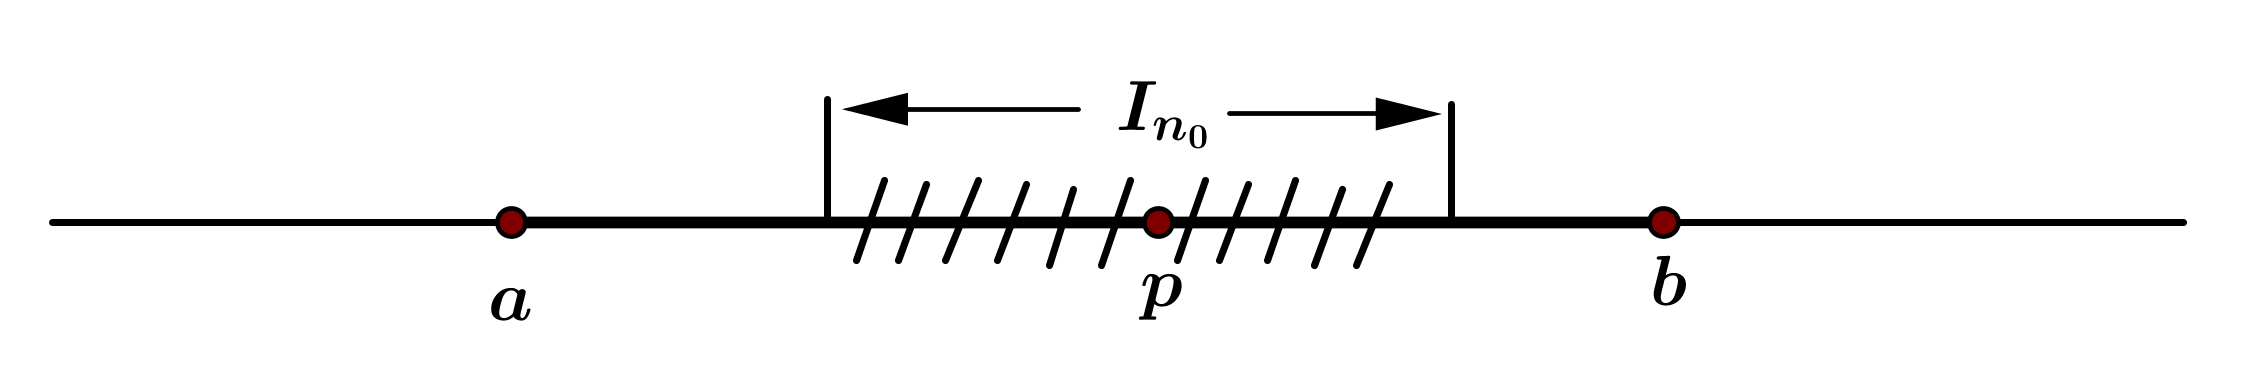
\includegraphics[width=.55\textwidth]{bolzano.png}
\caption{Bolzano}
\end{figure}

Since $I_{n_0}$ contains an infinite number of points of $A$, so does the open interval $S_p$. Thus each open interval containing $p$ contains points of $A$ other than $p$, i.e. $p$ is a limit point of $A$.
\end{proof}

\newpage
\subsection{Exercise}
Let $(X,d)$ be a metric space and let $A$ be a subset of $X$.
\begin{exer}\label{021}
Show that $A$ is open iff the compliment $A^c$ is closed.
\end{exer}

\begin{exer}\label{022}
Suppose $X$ has finitely many points. Prove that for every $x\in X$, the singleton set $\{x\}$ is open.
\end{exer}

\begin{exer}\label{023}
\end{exer}

\newpage
\subsection*{Solution}
\begin{proof}[Solution (\ref{021})]
$(\Rightarrow)$ Suppose $A$ is open. \\
Let $x$ be a limit point of $A^c$. Then every neighborhood $N$ of $x$ contains a point of $A^c$. Then $x$ is not an interior point of $A$ ($ x\in N\subsetneq A$). Since $A$ is open, this implies $x\in A^c$. Hence, $A^c$ contains all of its limit points(since $x$ was arbitrary). Therefore $A^c$ is closed.\\
$(\Leftarrow)$ Suppose $A^c$ is closed.\\
Let $x\in A$. This implies $x\notin A^c$ and $x$ is not a limit point of $A^c$($A^c$ is is closed). Then there exists a neighborhood $N$ of $x$ such that $A^c\cap N=\emptyset$. Hence $N\subset A$. Therefore, $A$ is open(by definition).
\end{proof}
\begin{proof}[Solution (\ref{022})]
For arbitrary $x\in X$ define $r(x)=\min\{d(x,y):y\in X,\ y\neq x\}$. Since all $d(x,y)>0$ when $x\neq y$, $r(x)$ is a minimum of finitely many positive numbers(since there are finitely many points). So $r(x)>0$. Consider the open ball $B(x,r(x))$. Now, suppose $y\in B(x,r(x))$ and $y\neq x$. Then by definition of being in the ball $d(x,y)<r(x)$ but $r(x)\leq d(x,y)$ by definition of $r(x)$. This is a contradiction, so $B(x,r(x))=\{x\}$. Therefore, as $x$ was arbitrary the set $\{x\}$ is open for any $x\in X$.
\end{proof}
\begin{proof}[Solution (\ref{023})]
Exercise.
\end{proof}

\newpage
\section{Compact sets}

\subsection{Definition}

\begin{defn}[\textbf{\color{blue}{Cover}}]
An open cover of a set $E$ in a metric space $X$ is a collection $\{G_{\alpha}\}$ of open subset of $X$ such that $E\subset \bigcup_{\alpha}G_{\alpha}$.
\end{defn}

\begin{defn}[\textbf{\color{blue}{Compact}}]
A subset $K$ of a metric space $X$ is said to be compact if every open cover of $K$ contains a finite subcover.
\end{defn}

\begin{defn}[\textbf{\color{blue}{Sequentially Compact}}]
A subset of a metric space is called (sequentially) compact if every sequence in the subset has a convergent subsequence.
\end{defn}

\begin{defn}[\textbf{\color{blue}{Least Upper Bound Axiom}}]
If $A$ is a set of real numbers bounded from above, then $A$ has a least upper bound, i.e. $\sup (A)$ exists.
\end{defn}

\begin{exmp}
Show that the set $E=\{0,1,\frac{1}{2},\frac{1}{3},\frac{1}{4},\ldots\}$ is compact.
\end{exmp}
\begin{proof}[Solution]
We need to show every open cover of $E$ has a finite subcover.\\
Let $E\subset U_{\alpha}$, where $U_{\alpha}$ is open set. Then $0$ must be in some $U_{\alpha_0}$. Since $U_{\alpha_0}$ open there exists $\delta>0$ such that $(-\delta,\delta)\subset U_{\alpha_0}$. In particular, $\frac{1}{n}$ in $U_{\alpha_0}$ if $n>\frac{1}{\delta}$. Let $N$ be the largest integer in $\frac{1}{\delta}$, and let $\alpha_i, i=1,\ldots,N$ be such that $\frac{1}{i}\in U_{\alpha_i}$. Then  $E\subset \bigcup_{i=1}^{n} U_{\alpha_i}$.
\end{proof}
\subsection{Facts}

\begin{thm}\label{subslimuniq}
In a metric space, any Cauchy sequence having a convergent subsequence is itself convergent, with the same limit.
\end{thm}
\begin{proof}
Suppose $\{x_n\}$ is a Cauchy sequence in a metric space $(X, d)$. Let $\{x_{n_k}\}$ be a convergent subsequence of $\{x_n\}$ with limit $x$. Then for any $\varepsilon> 0$, there exists $N_1 > 0$ such that
\[k > N_1\Rightarrow d(x_{n_k}, x) <\frac{\varepsilon}{2}.\]
Since $\{x_n\}$ is a Cauchy sequence, there also exists $N_2 > 0$ such that
\[m, n > N_2\Rightarrow d(x_n, x_m) <\frac{\varepsilon}{2}.\]
Let $N = \max\{N_1, N_2\}$ and choose $k > N$. Then $n_k \ge k > N$ and so
\[n > N\Rightarrow d(x_n, x)\le d(x_n, x_{n_k}) + d(x_{n_k}, x) < \frac{\varepsilon}{2}+\frac{\varepsilon}{2}=\varepsilon.\]
Thus $\{x_n\}$ converges to $x$.
\end{proof}

\begin{thm}
Compact subsets of a metric spaces are closed.
\end{thm}
\begin{proof}
Suppose $S$ is a compact subset of a metric space $X$. Let $\{x_n\}$ be a sequence in $S$ that converges to a point $x\in X$. This implies, in particular, that $\{x_n\}$ is a Cauchy sequence. Since $S$ is compact, $\{x_n\}$ has a subsequence which converges to a point $y\in S$. Then, by Theorem (\ref{subslimuniq}), we know that $\{x_n\}$ is convergent in S and so $x = y\in S$ (by uniqueness of limits). Hence $S$ is closed.
\end{proof}

\begin{thm}
Closed subsets of a compact sets are compact.
\end{thm}
\begin{proof}
Exercise
\end{proof}

\begin{exmp}[\color{red}{\textbf{Counter-example\footnote{Bartle, pp. 320}}}]
Let $K :=\{x_1,x_2,\ldots,x_n\}$ be a finite subset of $\Bbb R$. If $\mathcal{G}= \{\mathcal{G}_{\alpha}\}$ is an open cover of $K$, then each $x_i$ is contained in some set $\mathcal{G}_{\alpha_i}$ in $\mathcal{G}$. Then the union of the sets in the collection $\{\mathcal{G}_{\alpha_1},\mathcal{G}_{\alpha_2},\ldots, \mathcal{G}_{\alpha_n}\}$ contains $K$, so that it is a finite subcover of $\mathcal{G}$. Since $\mathcal{G}$ was arbitrary, it follows that the finite set $K$ is compact.
\end{exmp}

\begin{exmp}[\color{red}{\textbf{Counter-example}}]
Let $A_1,A_2,A_3,\ldots$ be the following sequence of open-closed intervals:
$$A_1=(0,1],A_2=(0,1/2],\ldots,A_k=(0,1/k],\ldots$$
Now the sequence of intervals is nested, i.e. each interval contains the succeeding interval; $A_1\supset A_2\supset \cdots.$ But the intersection of the intervals is empty, i.e.,
$$A_1\cap A_2\cap \cdots \cap A_k\cap \cdots=\emptyset$$
Thus there exists no point common to every interval.
\end{exmp}

\begin{exmp}[\color{red}{\textbf{Counter-example}}]
Let $A_1,A_2,A_3,\ldots$ be the following sequence of closed infinite intervals:
$$A_1=[1,\infty),A_2=[2,\infty),\ldots,A_k=[k,\infty),\ldots$$
Now $A_1\supset A_2\supset \cdots$, i.e. the sequence of intervals is nested. But there exists no point common to every interval, i.e.
$$A_1\cap A_2\cap \cdots \cap A_k\cap \cdots=\emptyset$$
\end{exmp}

\begin{thm}[\textbf{Heine-Borel}]
Let $I_1=[c_1,d_1]$ be a closed(bounded) subset of $\Bbb R$ which is covered by $\mathcal{G}=\{(a_1,b_i):i\in I\}$ of open intervals. Then $\mathcal{G}$ contains a finite subclass which also covers $I_1$.
\end{thm}
\begin{proof}
Assume that no finite subclass of $\mathcal{G}$ covers $I_1$. We bisect $I_1=[c_1,d_1]$ at $\frac{1}{2}(c_1+d_1)$ and consider the two closed intervals
\begin{align}\label{borel1}
\biggl[c_1, \frac{1}{2}(c_1+d_1)\biggl]\text{ and } \biggl[\frac{1}{2}(c_1+d_1),d_1\biggl]
\end{align}
At least one of this two intervals can not be covered by a finite subclass of $\mathcal{G}$ or else the whole interval $I_1$ will be covered by a finite subclass of $\mathcal{G}$. Let $I_2=[c_2,d_2]$ be one of the two intervals in (\ref{borel1}) which can not be covered by a finite subclass of $\mathcal{G}$, we now bisect $I_2$. As before one of the two intervals
\begin{align*}
\biggl[c_2, \frac{1}{2}(c_2+d_2)\biggl]\text{ and } \biggl[\frac{1}{2}(c_2+d_2),d_2\biggl]
\end{align*}
can not be covered by a finite subclass of $\mathcal{G}$. Call that interval $I_3$.\\
We continue this procedure and obtain a sequence of nested intervals $I_1\supset I_2\supset I_3\supset\ldots$ such that each interval $I_n$ can not be covered by a finite subclass of $\mathcal{G}$ and $\lim |I_n|=0$ where $|I_n|$ denotes the length of the interval $I_n$.\\
By the nested interval property of the real numbers (\ref{nest}) there exists a point $p$ in each interval $I_n$. In particular , $p\in I_1$, since $\mathcal{G}$ is a cover of $I_1$, there exists an open interval $(a_{i_0},b_{i_0})$ in $\mathcal{G}$ which contains $p$. Hence $a_{i_0}<p<b_{i_0}$. Since $\lim |I_n|=0$
\begin{align*}
\exists n_0\in \Bbb N \qquad\text{such that}\qquad |I_{n_0}|<\min(p-a_{i_0},b_{i_0}-p)
\end{align*}
Then, as indicated in the diagram below, the interval $I_{n_0}$ is a subset of the interval $(a_{i_0},b_{i_0})$ in $\mathcal{G}$.
\begin{figure}[hbt!]
\centering
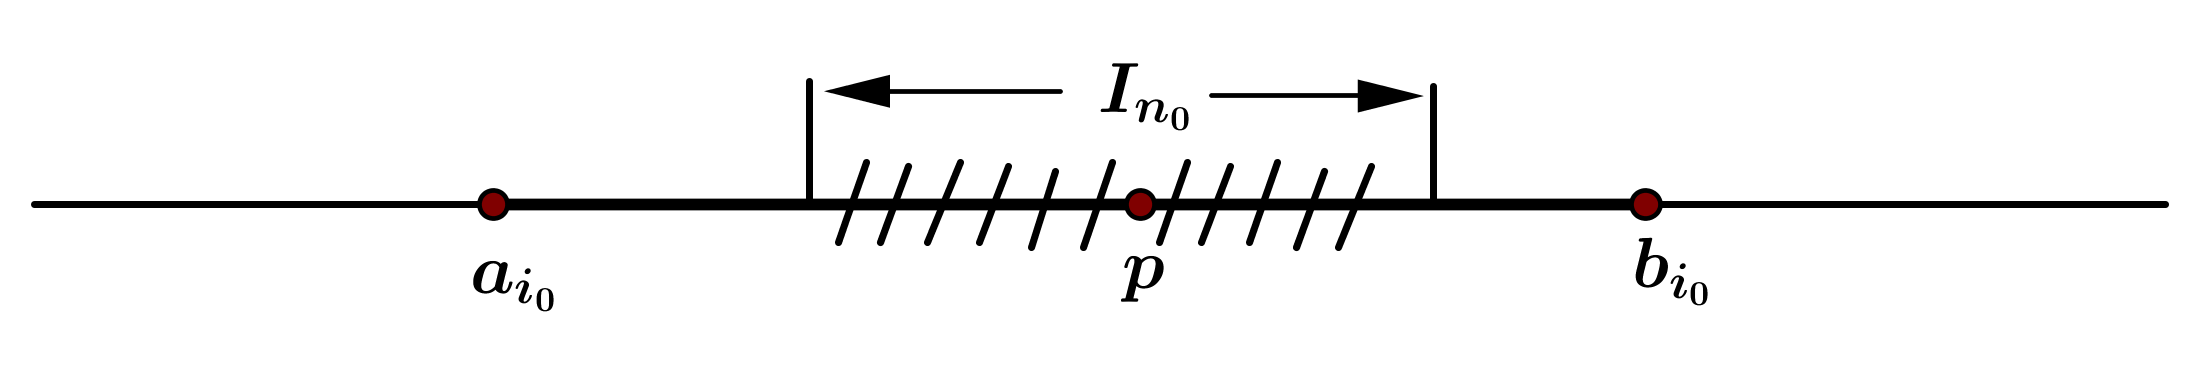
\includegraphics[width=.6\textwidth]{borel.png}
\caption{Borel}
\end{figure}

But this contradicts our choice of $I_{n_0}$. Thus the original assumption that no finite subclass of $\mathcal{G}$ covers $I_1$ is false and the theorem is true.
\end{proof}
\begin{rem}\color{red} Any closed and bounded set is not necessarily compact.\\
Let $\Bbb Q$, the set of rational numbers, as a metric space, with $d(p,q)=|p-q|$. Let $E$ be the set of all $p\in \Bbb Q$ such that $2<p^2<3$. $E$ is close and bounded in $\Bbb Q$ but $E$ is not compact.\\
But if $A\subset \Bbb R^k$ is closed and bounded, then $A$ is compact(Heine-Borel theorem).
\end{rem}

\begin{exmp}[\color{red}{\textbf{Counter-example}}]
Consider the open and bounded interval $A=(0,1)\subset \Bbb R^1$. Observe that the class
\begin{align}
\mathcal{G}=\biggl\{G_n=\biggl(\frac{1}{n+2},\frac{1}{n}\biggl):n\in \Bbb N\biggl\}
\end{align}
of open intervals covers $A$. i.e.
\begin{align*}
A\subset \biggl(\frac{1}{3},1\biggl)\cup\biggl(\frac{1}{4},\frac{1}{2}\biggl)\cup\biggl(\frac{1}{5},\frac{1}{3}\biggl)\cup\cdots
\end{align*}
But the union of no finite subclass of $\mathcal{G}$ contains $A$.
\end{exmp}

\begin{exmp}[\color{red}{\textbf{Counter-example}}]
Consider the  closed infinite interval $A=[1,\infty)$. The class
\begin{align}
\mathcal{G}=\{(0,2),(1,3),(2,4),\ldots\}
\end{align}
of open intervals covers $A$ but no finite subclass does.
\end{exmp}

\newpage
\subsection{Exercise}

\begin{exer}\label{031}
Show that a compact metric space $(X,d)$ is complete.
\end{exer}

\begin{exer}\label{032}
\end{exer}

\begin{exer}\label{033}
\end{exer}

\newpage
\subsection*{Solution}
\begin{proof}[Solution (\ref{031})]
Since $X$ is a compact metric space it is sequentially compact.\\ Let $x_n$ be a Cauchy sequence in the metric space $X$. Since $X$ is sequentially compact there is a convergent subsequence $x_{n_k}\to x \in X$.

All that now remains to be shown is that $x_n \to x$. Since $x_{n_k}\to x$ there is $N_1$ with $n_k \ge N_1$ implies $|x_{n_k}-x|<{\varepsilon\over 2}$. Let $N_2$ be such that $n,m\ge N_2$ implies $|x_n-x_m|<{\varepsilon \over 2}$.

Then $n>N=\max(N_1,N_2)$ implies
$$ |x_n-x|\le |x_n-x_N|+|x_N-x|<\varepsilon$$
Hence $X$ is complete.
\end{proof}

\begin{proof}[Solution (\ref{032})]
\end{proof}

\begin{proof}[Solution (\ref{033})]
Exercise.
\end{proof}

\newpage
\section{Sequences}

\subsection{Definition}
\begin{defn}[\textbf{\color{blue}{Sequence}}]
A sequence is a function whose domain is the set of natural numbers. That is $f:\Bbb N\rightarrow \Bbb R$.
\end{defn}
\begin{notn}
We usually denote a sequence by
\[\{a_1,a_2,a_3,\ldots\},\qquad \text{ or }\qquad\{a_k\}\]
\end{notn}

\begin{defn}[\textbf{\color{blue}{Subsequence}}]
A sequence $\{a_{n_k}\}=\{a_{n_1},a_{n_2},a_{n_3},\ldots\}$ is a a subsequence of $\{a_k\}$ iff $n_1,n_2,n_3,\ldots$ are positive integers, with  $n_1<n_2<n_3<\cdots$.
\end{defn}

\begin{defn}[\textbf{\color{blue}{Bounded}}]
A sequence $\{a_k\}$ is bounded if there is $M>0$ such that $|a_k|<M$ for all $k\in \Bbb N$.
\end{defn}

\begin{defn}[\textbf{\color{blue}{Convergent}}]
A sequence $\{a_k\}$ converges to $a\in \Bbb R$;
\[\lim_{k\rightarrow \infty} a_k=a\]
iff for every $\varepsilon>0$ there exists an $N\in \Bbb N$ such that
\[k>N \qquad \Rightarrow \qquad |a_k-a|<\varepsilon.\]
\end{defn}

\begin{defn}[\textbf{\color{blue}{Cauchy criterion}}]
A sequence $\{a_k\}$ is Cauchy if for every $\varepsilon>0$ there exists an $N\in \Bbb N$ such that
\[m,n>N \qquad \Rightarrow \qquad |a_m-a_n|<\varepsilon.\]
\end{defn}

\begin{exmp}[\color{red}{\textbf{Counter-example}}]
Consider $\Bbb Q$ with the usual metric $d=|y-x|,\forall x,y\in\Bbb Q$. Show that $(\Bbb Q,d)$ is not complete.
\end{exmp}
\begin{proof}[Solution]
Consider the sequence defined by
\begin{align} x_1=1,\qquad x_{n+1}=\frac{x_n}{2}+\frac{1}{x_n},
\end{align}
which is Cauchy but it doesn't converge in $\Bbb Q$. If the sequence converges say to $x$, then $x_{n+1}\to x$ and $x_n\to x$ and hence $x^2=2$.
\end{proof}
\subsection{Facts}

\begin{thm}[\textbf{Uniqueness}]
If $\{a_k\}$ converges, then the limit is uniquely determined.
\end{thm}

\begin{proof}(Contradiction)\\
Suppose $\lim a_k=a$ and $\lim a_k=b$, with $a\neq b$.\\
We have for every $\varepsilon>0$, in particular $\varepsilon=\frac{1}{4}|b-a|$ there is $N_{a}(\varepsilon)$ such that
\[k>N_{a}(\varepsilon) \qquad \Rightarrow \qquad |a_k-a|<\frac{1}{4}|b-a|.\]
Similarly, we have
\[k>N_{b}(\varepsilon) \qquad \Rightarrow \qquad |a_k-b|<\frac{1}{4}|b-a|.\]
Now,
\[|a-b|=|a-a_k+a_k-b|\leq |a-a_k|+|a_k-b|\leq \frac{1}{4}|b-a|+\frac{1}{4}|b-a|=\frac{1}{2}|b-a|\]
This implies $|b-a|=0$, thus $a=b$ a contradiction to our assumption that $a\neq b$.
\end{proof}

\begin{thm}\label{covergbound}
If $\{a_n\}$ converges to a limit $a\in \Bbb R$, then $\{a_n\}$ is bounded.
\end{thm}

\begin{proof}
Assume $\{a_n\}$ converges to $a$. Then by definition we have, for $\varepsilon>0$ there is $N>0$ such that \\
\[n>N\qquad \Rightarrow \qquad |a_n-a|<\varepsilon\]
In particular let $\varepsilon=1.$ Thus, $|a_n-a|<1$ which implies $|a_n|<1+|a|$ so for $n>N$ the sequence $\{a_n\}$ is bounded by $1+|a|$. Otherwise $\{a_n\}$ is bounded by the $\max\{|a_1|,|a_2|,\ldots,|a_N|\}$. Put
\[M=\max\{|a_1|,|a_2|,\ldots,|a_N|,1+|a|\}\]
Then $|a_n|<M$ for all $n\in \Bbb N$. Therefore $\{a_n\}$ is bounded.
\end{proof}
\begin{exmp}[\color{red}{\textbf{Counter-example}}]
The converse of theorem (\ref{covergbound}) may not be true. Take for example(usually) the sequence
\begin{align*}
\{(-1)^n\}
\end{align*}
which is bounded but not convergent.
\end{exmp}

\begin{thm}
If $\{a_k\}$ converges to $a$, and if $\{a_{n_k}\}$ is a subsequence of $\{a_k\}$ then $\{a_{n_k}\}$ converges to $a$.
\end{thm}

\begin{proof}
We first show that
\[n_k\geq k\qquad \text{ for all } k\in\Bbb N.\]
For $k=1$, it is trivial $n_1\geq 1$. Now we assume $n_k\geq k$. Since $n_{k+1}>n_k$, hence $n_{k+1}\geq n_k+1$. Then we have
\[n_{k+1}\geq n_k+1\geq k+1.\]
Since $\{a_k\}$ converges to $a$, we have, for every $\varepsilon>0$, there is $N\in \Bbb N$ such that
\[\qquad |a_k-a|<\varepsilon\qquad \text{ for all } k\geq N.\]
Hence
\[\qquad |a_{n_k}-a|<\varepsilon \qquad \text{ for all }n_k\geq N.\]
Since $n_k\geq k$, we have also
\[|a_{n_k}-a|<\varepsilon \qquad \text{ for all }k \geq N.\]

\end{proof}

\begin{thm}
Every convergent sequence is Cauchy sequence.
\end{thm}

\begin{proof}
Exercise
\end{proof}

\begin{thm}
Every Cauchy sequence of real numbers is convergent.
\end{thm}

\begin{proof}
Exercise
\end{proof}

\newpage
\subsection{Exercise}
\begin{exer}\label{041}
Show that $\{x_n\}$ defined by
\[x_n = 1 +\frac{1}{2}+\cdots +\frac{1}{n}\]
is divergent.
\end{exer}

\begin{exer}\label{042}
Show that $\{x_n\}$ defined by
\[x_n = 1 +\frac{1}{2}+ \cdots +\frac{1}{n}-\ln(n)\]
is convergent.
\end{exer}

\begin{exer}\label{043}
\end{exer}

\newpage
\subsection*{Solution}
\begin{proof}[Solution (\ref{041})]
We have
\[x_{2n}- x_n =\frac{1}{n+1}+\frac{1}{n+2} +\cdots +\frac{1}{2n}\]
for any $n\ge1$. So
\[\frac{1}{n+n}+\frac{1}{n+n} +\cdots +\frac{1}{2n}\leq x_{2n}- x_n\]
or $\frac{1}{2} \leq x_{2n}-x_n$. This clearly implies that $\{x_n\}$ fails to be Cauchy. Therefore it diverges.
\end{proof}
\begin{proof}[Solution (\ref{042})]
Recall the integral definition of the logarithm function. In particular, we have
\[\ln(x) = \int_1^x \frac{1}{t}dt.\]
In this case if $0 < a < b$, then we have
\[\frac{b-a}{b}\leq \int_a^b\frac{1}{t} dt\leq \frac{b-a}{a}.\]
Since
\[\ln(n) = \int_1^n\frac{1}{t}dt = \sum_{k=1}^{n-1}\int_k^{k+1}\frac{1}{t} dt,\]
we get
\[\ln(n)\leq \sum_{k=1}^{n-1}\frac{k+1-k}{k} = 1 +\frac{1}{2}+\cdots +\frac{1}{n-1}.\]
Hence
\[x_n = 1 +\frac{1}{2}+\cdots +\frac{1}{n}-\ln(n) = 1 + \frac{1}{2}+\cdots +\frac{1}{n-1}-\ln(n)+\frac{1}{n}>0.\]
On the other hand, we have
\[x_{n+1}-x_n =\frac{1}{n+1}-\ln(n + 1) + \ln(n) = \frac{1}{n + 1}-\int_n^{n+1}\frac{1}{t}dt < 0.\]
These two inequalities imply that $\{x_n\}$ is decreasing and bounded below by $0$. Therefore $\{x_n\}$ is convergent\footnote{Its limit is $\gamma= 0.57721\ldots$, which is known as the Euler constant.}.
\end{proof}
\begin{proof}[Solution (\ref{043})]
Exercise.
\end{proof}

\newpage
\section{Continuity}

\subsection{Definition}
\begin{defn}[\textbf{\color{blue}{Continuous}}]
A function $f:\Bbb R\rightarrow \Bbb R$ is continuous at a point $x_0$ iff for every $\varepsilon>0$ there is a $\delta>0$ such that
\[|x-x_0|<\delta\qquad \Rightarrow \qquad |f(x)-f(x_0)|<\varepsilon\]
which is equivalent to
\begin{align}
x\in (x_0-\delta,x_0+\delta)\qquad \Rightarrow \qquad f(x)\in (f(x_0)-\varepsilon,f(x_0)+\varepsilon).
\end{align}
which is again equivalent to $f[(x_0-\delta,x_0+\delta)] \text{ is contained in }(f(x_0)-\varepsilon,f(x_0)+\varepsilon).$
\end{defn}

\subsection{Facts}
\begin{thm}[\color{DarkGreen}{\textbf{Characterization}}]
A function $f:X\to Y$ is continuous iff the inverse image of every open set is open.
\end{thm}
\begin{proof}[Formal Proof]
Suppose $f$ is continuous on $X$ and $V$ is an open set in $Y$. We have to show that every point of $f^{-1}(V)$ is an interior point of $f^{-1}(V)$. So, suppose  $p\in X$ and $f(p)\in V$. Since $V$ is open, there exists $\varepsilon>0$ such that $y\in V$ if $d_Y(f(p), y) < \varepsilon$ ; and since $f$ is continuous at $p$, there exists $\delta > 0$
such that $d_Y(f(x), f(p)) < \varepsilon$ if $d_X(x, p) < \delta$. Thus $x\in f^{-1}(V)$ whenever $d_X(x, p) <\delta$. \\
Conversely, suppose $f^{-1}(V)$ is open in $X$ for every open set $V$ in $Y$. Fix $p\in X$ and $\varepsilon > 0$, let $V=\{y\in Y:d_Y(y, f(p)) < \varepsilon\}$.
Then $V$ is open ; hence $f^{-1}(V)$ is open ; hence there exists $\delta> 0$ such that $x\in f^{-1}(V)$ whenever $d_X(p, x) < \delta$. But if $x \in f^{-1}(V)$, then $f(x)\in V$, so that $d_Y(f(x),f(p)) < \varepsilon$.
\end{proof}

\begin{proof}[Informal Proof]
\color{red}{Note that even if $f$ is not a bijective( and doesn't have an inverse function $f^{-1}$) the set $f^{-1}(B)=\{x\in X|f(x)\in B\}$ still exists.}\\
\color{black}
$(\Rightarrow)$ Take $x\in f^{-1}(B)$. Then $f(x)=y\in B$. Since $B$ is open the point $y$ has an $\varepsilon-$neighbourhood $\subset B$. Then from the definition of continuity this $\varepsilon-$neighbourhood contains the image of some $\delta-$neighbourhood of $x$. Since $f(V)\subset B$, we have $V\subset f^{-1}(B)$ and so $x$ has this $\delta-$neighbourhood $\subset f^{-1}(B).$ Hence $f^{-1}(B)$ is open in $X$.\\
$(\Leftarrow)$ To show $f$ is continuous at $x_0\in X$, take $B$ to be an $\varepsilon-$neighbourhood of $y\in Y$. Then $f^{-1}(B)$ is open in $X$ and so $x_0$ has $\delta-$neighbourhood in $f^{-1}(B)$. This $\delta-$neighbourhood is mapped inside the $\varepsilon-$neighbourhood of $f(x_0)$. Hence $f$ is continuous at $x_0$.
\end{proof}

\begin{cor}
A function $f:X\to Y$ is continuous iff the inverse image of every closed set is closed.
\end{cor}
\begin{proof}
The proof follows, since a set is closed iff its compliment is open, and $f^{-1}(E^c)=[f^{-1}(E)]^c$ for every $E\subset Y$.
\end{proof}

\begin{rem}\color{red}
Openness and closedness are preserved under inverse, continuous images. Be aware that these properties are not preserved under continuous, direct images; even if $f$ is continuous, the image $f(U)$ of an open set $U$ need not be open, and the image $f(F)$ of a closed $F$ need not be closed.
\end{rem}
\begin{exmp}[\color{red}{\textbf{Counter-example}}]
Let $f,g : \Bbb R\to \Bbb R$ be the continuous functions defined by
\[f(x) = x^2\qquad \text{and}\qquad g(x) = \arctan x\]
The set $\Bbb R$ is both open and closed, but $f(\Bbb R)$ equals $[0, \infty)$ which is not open, and $g(\Bbb R)$ equals $(-\frac{\pi}{2}, \frac{\pi}{2})$ which is not closed. Hence the continuous image of an open set need not be open, and the continuous image of a closed set need not be closed.
\end{exmp}

\begin{thm}
Suppose $f$ is a continuous mapping of a compact metric space $X$ into a metric space $Y$. Then $f(X)$ is compact.
\end{thm}

\begin{proof}
Let $\{V_{\alpha}\}$ be any open cover of $f(X)$. Since $\{v_{\alpha}\}$ is open in $Y$, $f^{-1}(V_{\alpha})$ is open in $X$. Since $X$ is compact there are finitely many $\alpha_i$'s such that
\begin{align*}
X&\subset f^{-1}(V_{\alpha_1})\cup f^{-1}(V_{\alpha_2})\cup\cdots \cup f^{-1}(V_{\alpha_n})\\
\Rightarrow X &\subset \bigcup_{i=1}^{n}f^{-1}(V_{\alpha_i})=f^{-1}\biggl(\bigcup_{i=1}^{n}V_{\alpha_i}\biggl)\\
\Rightarrow f(X)&\subset f\biggl(f^{-1}\biggl(\bigcup_{i=1}^{n}V_{\alpha_i}\biggl)\biggl)\\
\Rightarrow f(X)&\subset \bigcup_{i=1}^{n}V_{\alpha_i}
\end{align*}
Hence, $f(X)$ is compact.
\end{proof}

\begin{thm}
If $f$ is a continuous mapping of a metric space $X$ into a metric space $Y$, and if $E$ is a connected subset of $X$, then $f(E)$ is connected.
\end{thm}

\begin{proof}
Assume, on the contrary, that $f(E)$ is not connected i.e. $f(E) = A \cup B$, where $A$ and $B$ are nonempty separated subsets of $Y$. Put $G = E \cap f^{-1}(A),\ H = E \cap f^{-1}(B)$.\\
Then $E = G \cup H$, and neither $G$ nor $H$ is empty.\\
Since $A \subset \overline{A}$ (the closure of A ), we have $G\subset f^{-1}(\overline{A})$ ; the latter set is closed, since $f$ is continuous; hence $G \subset f^{-1}(\overline{A})$. It follows that $f(\overline{G})\subset \overline{A}$.
Since $f(H) = B$ and $\overline{A}\cap B$ is empty, we conclude that $\overline{G}\cap H$ is empty.\\
The same argument shows that $G \cap \overline{H}$ is empty. Thus $G$ and $H$ are separated. This contradict the fact that $E$ is connected.
\end{proof}

\newpage
\subsection{Exercise}
\begin{exer}\label{051}
Let $I=[0,1]$ be the closed unit interval. Suppose $f$ is a mapping of $I$ into $I$. Prove that $f(x)=x$ for at least one $x\in I$.
\end{exer}

\begin{exer}\label{052}
Let $f$ be a continuous real function on a metric space $X$. Let $Z(f)$ (the zero set of $f$) be the set of all $p\in X$ at which $f(p)= 0$. Prove that $Z(f)$ is closed.
\end{exer}

\begin{exer}\label{053}
\end{exer}


\newpage
\subsection*{Solution}
\begin{proof}[Solution (\ref{051})]
If $f(0)=0$ or $f(1)=1$, we are done. If not, then $0<f(0)$ and $f(1)<1$. Hence the continuous function $g(x)=x-f(x)$ satisfies $g(0)<0<g(1)$. Then by Intermediate value theorem, there must be a point $x\in (0,1)$ where $g(x)=0$.
\end{proof}
\begin{proof}[Solution (\ref{052})]
$Z(f)=f^{-1}(\{0\})$, which the inverse image of a closed set. Hence $Z(f)$ is closed.
\end{proof}
\begin{proof}[Solution (\ref{053})]
Exercise.
\end{proof}
\newpage

\section{Sequence and Series of Functions}


\subsection{Definition}

\begin{defn}[\textbf{\color{blue}{Pointwise convergence}}]
A sequence of functions $\{f_n : D \to \Bbb R\}$ defined on a subset $D\subset R$ converges pointwise on $D$ if for each $x\in D$ the sequence of numbers $\{f_n(x)\}$ converge. If $\{f_n\}$ converges pointwise on $D$, then we define $f : D\to \Bbb R$ with $f(x) = \lim_{n\to\infty}f_n(x)$ for each $x\in D$. We denote this symbolically by $f_n\to f$ on $D$.
\end{defn}

\begin{defn}[\textbf{\color{blue}{Uniform convergence}}]
A sequence of functions $\{f_n : D \to \Bbb R\}$ defined on a subset $D\subset R$ converges uniformly on $D$ to a function $f$ such that for every $\varepsilon> 0$ there is a number $N\in \Bbb N$ such that
$$|f_n(x)-f(x)| < \varepsilon \qquad \text{for all } x \in D, n \geq N.$$
We denote this type of convergence symbolically by $f_n\rightrightarrows f$ on $D$.
\end{defn}

\begin{defn}
If $\{f_n\}$ is a sequence of functions defined on $D$, the series $\sum_{n=0}^{\infty}f_n$ is said to converge pointwise(respectively, uniformly) on $D$ if and only if the sequence $\{s_n\}$ of partial sums, given by
$$s_n(x) =\sum_{k=0}^{n}f_k(x),$$
converges pointwise (respectively, uniformly) on $D$.
\end{defn}

\begin{defn}[\textbf{\color{blue}{Pointwise bounded}}]
Let $\{f_n\}$ be a sequence of functions defined on a set $E$. We say that $\{f_n\}$ is pointwise bounded on $E$ if the sequence $\{f(x)\}$ is bounded for every $x\in E$, that is, if there exists a finite-valued function $\phi$ defined on $E$ such that
$$|f_n(x)| < \phi(x) \qquad (x\in E, n = 1, 2, 3,\ldots).$$
\end{defn}
\begin{defn}[\textbf{\color{blue}{Uniformly bounded}}]
$\{f_n\}$ is uniformly bounded on $E$ if there exists a number $M$ such that
$$|f_n(x)|< M\qquad  (x\in E, n = 1, 2, 3,\ldots).$$
\end{defn}
\begin{defn}[\textbf{\color{blue}{Equicontinuous}}]
A family $\mathcal{F}$ of functions $f$ defined on a set $E$ in a metric space $X$ is said to be equicontinuous on $E$ if for every $\varepsilon > 0$ there exists a $\delta> 0$ such that
$$|f(x) - f(y)| < \varepsilon$$
whenever $d(x, y) < \delta,\ x,y\in E$, and $f\in \mathcal{F}$.
\end{defn}
\subsection{Facts}

\begin{thm}[\textbf{Uniform Cauchy Criterion}]
If $\{f_n\}$ is a sequence of functions defined on $A$, then $\{f_n\}$ is uniformly convergent on $D$ if and only if for $\varepsilon > 0$, there exists $N \in\Bbb N$ such that for any $m, n > N$
$$\sup_{x\in D}|f_n(x)-f_m(x)| < \varepsilon.$$
\end{thm}
\begin{proof}
$(\Rightarrow)$ Suppose $f_n\rightrightarrows f$, then given $\varepsilon > 0$, we can find an integer $N$ such that
\[m\ge N \rightarrow |f_m(x)-f(x)| < \frac{\varepsilon}{2}\]
for all $x\in D$. If $m, n\ge N$, then
\[|f_m(x)-f_n(x)| \le |f_n(x)-f(x)| + |f(x)-f_n(x)| < \frac{\varepsilon}{2}+\frac{\varepsilon}{2}=\varepsilon\]
for any $x \in D$.\\
$(\Leftarrow)$ If given some $\varepsilon > 0$, we can find an $N$ such that for any $m, n\ge N$ we have
\[\sup_{x\in D} |f_n(x)-f_m(x)| < \varepsilon.\]
Hence for any $x\in D$, $\{f_n(x)\}$ is a Cauchy sequence in $\Bbb R$ which implies $f_n(x)$ converges to $f(x)$. Let us prove that $\{f_n\}$ converges uniformly to $f$ on $D$. Indeed, let $\varepsilon > 0$. By the uniform Cauchy criterion, there exists $N\in \Bbb N$ such that for all $n, m\ge N$, we have $\sup_{x\in D} |f_n(x)-f_m(x)| \le \varepsilon/2$. Fix $n\ge N$. Then
\[|f_n(x)-f(x)| = \lim_{m\to\infty}|f_n(x)-f_m(x)|\le \frac{\varepsilon}{2}\]
for any $x\in D$. Hence
\[\sup_{x\in D}|f_n(x)-f(x)| \le \frac{\varepsilon}{2}< \varepsilon.\]
This implies $f_n\rightrightarrows f$ on $D$.
\end{proof}

\begin{thm}[\textbf{M-test}]
A sequence of functions $\{f_n\}$ defined on $D$ is uniformly convergent on $U\subset D$ to $f : U\to\Bbb R$ if and only if $\lim_{n\to\infty} M_n = 0$, where
$$M_n:=\sup\{|f_n(x)-f(x)| : x \in U\}, n \in\Bbb N.$$
\end{thm}
\begin{proof}
$(\Rightarrow)$ Suppose $f_n \rightrightarrows f$ on $U$. Then given $\varepsilon > 0$, there exists $N\in\Bbb N$ such that
\[|f_n(x)-f(x)| < \varepsilon\ \forall n\ge N\ \forall x\in U.\]
Hence,
\[a_n := \sup\{|f_n(x)-f(x)| : x\in U, n\ge N\} <\varepsilon\]
and therefore $\lim_{n\to\infty}a_n = 0$.
$(\Leftarrow)$ Suppose $\lim_{n\to\infty}a_n = 0$. Then for large $n$ and $\forall x\in U$
\[|f_n(x)-f(x)| \le \sup\{|f_n(x)-f(x)| : x\in U\} < \varepsilon.\]
That is, $f_n\rightrightarrows f$ on $U$.
\end{proof}

\begin{thm}[\textbf{Weierstrass M-test}]
Suppose that $\{f_n\}$ is a sequence of functions defined on $D$ and $\{M_n\}$ is a sequence of nonnegative integers such that
$$|f_n(x)| \leq M_n,\ \forall x \in D, \forall n\in\Bbb N.$$
Show that if $\sum_{n=0}^{\infty} M_n$ converges, then $\sum_{n=0}^{\infty}f_n(x)$ converges uniformly on $D$.
\end{thm}
\begin{proof}
Let $s_n(x) =\sum_{k=0}^{n}f_k(x)$ be the $n^{th}$ partial sum. Since $\sum_{n=0}^{\infty}M_n$
converges, for all $\varepsilon > 0$, $\exists N$ such that if $n\ge m \ge N$, then
\[M_m+ M_{m+1} +\cdots + M_n < \varepsilon.\]
Thus if $n \ge m \ge N$, we have
\begin{align*}
|s_n(x) - s_m(x)| &= |f_{m+1}(x) + \cdots + f_n(x)|\\
                  &\le |f_{m+1}(x)| +\cdots + |f_n(x)|\\
                  &\le M_{m+1} +\cdots + M_n < \varepsilon
\end{align*}
for all $x\in D$. It follows (from uniform cauchy criterion) that $\{s_n\}$ converges uniformly on $D$. Hence $\sum_{n=0}^{\infty}f_n$ also converges uniformly on $D$.
\end{proof}

\begin{thm}
Assume that $f_n$ converges uniformly to $f$ on $[a, b]$ and that each $f_n$ is integrable. Then, $f$ is integrable
and
\[\lim_{n\to\infty}\int_a^b f_n=\int_a^b f\]
\end{thm}
\begin{proof}
Exercise
\end{proof}

\begin{thm}[\textbf{Termwise integration}]
If each function $f_n(x)$ is continuous on a closed interval $[a, b]$ and if the series $\sum_{n=1}^{\infty}f_n(x)$ converges uniformly on $[a, b]$, then we have
\[\sum_{n=1}^{\infty}\int_a^b f_n(x)dx =\int_a^b\sum_{n=1}^{\infty}f_n(x)dx\]
\end{thm}
\begin{proof}
Exercise
\end{proof}

\begin{thm}
Suppose that $\{f_n\}$ converges to $f$ on the interval $[a, b]$. Suppose also that $f'_n$ exists and is
continuous on $[a, b]$, and the sequence $\{f'_n\}$ converges uniformly on $[a, b]$. Then
\[\lim_{n\to\infty} f'_n(x) = f'(x)\]
for each $x\in [a, b]$.
\end{thm}
\begin{proof}
Exercise
\end{proof}

\begin{thm}[\textbf{Termwise differentiation}]
If each function $f_n(x)$ has the derivative $f'_n(x)$ at any point $x\in (a, b)$, if the series $\sum_{n=1}^{\infty}f_n(x)$ converges to at least one point $k\in (a, b)$, and if $\sum_{n=1}^{\infty}f'_n(x)$ converges uniformly on $(a, b)$ to a function $g(x)$, then $\sum_{n=1}^{\infty}f_n(x)$ converges uniformly on $(a, b)$ and is differentiable at any point $x\in (a, b)$, whose derivative is equal to $g(x)$. In other words, termwise differentiation is possible, i.e.,
\[\biggl(\sum_{n=1}^{\infty}f_n(x)\biggl)'=\sum_{n=1}^{\infty}f'_n(x)\]
\end{thm}
\begin{proof}
Exercise
\end{proof}

\begin{thm}[\textbf{Dini}]
Let $A \subset \Bbb R$ be a closed and bounded (and thus compact) set and $\{f_n\}$ be a sequence of continuous functions $f_n : A\to \Bbb R$ such that\\
a) $f_n(x) \geq 0$ for any $x\in A$,\\
b) $f_n\to f$ pointwise and $f$ is continuous,\\
c) $f_{n+1}(x) \leq f_n(x)$ for any $x \in A$, and any $n \in \Bbb N$.
Then $\{f_n\}$ converges to $f$ uniformly on $A$.
\end{thm}

\begin{proof}
Exercise
\end{proof}
\begin{thm}[\textbf{Arzela-Ascoli}]
Let $\{f_n\}$ be a sequence of functions defined on a compact set $K$. If $f_n$ is uniformly bounded and equicontinuous on $K$, then $f_n$ has a uniformly convergent subsequence.
\end{thm}
\begin{proof}
Exercise
\end{proof}

\begin{thm}[\textbf{Stone-Weierstrass}]
If $f$ is a continuous function on a closed interval $[a, b]$, then there exists a sequence of polynomials $P_n$ such that
$$\lim_{n\to\infty}P_n(x) = f(x)$$
uniformly on $[a, b]$.
\end{thm}
\begin{proof}
Exercise
\end{proof}

\newpage
\subsection{Exercise}
\begin{exer}\label{061}
Let $f_n(x) : [1, 2] \to \Bbb R$ be defined by
\[
f_n(x) = \frac{x}{(1 + x)^n}
\]
\begin{description}
  \item[(a)] Show that $\sum_{n=1}^{\infty}f_n(x)$ converges for $x\in [1, 2]$. Is the convergence is uniform?
  \item[(b)] Does the following hold:
   \[\int_{1}^{2}\biggl(\sum_{n=1}^{\infty}f_n(x)\biggl)dx=\sum_{n=1}^{\infty}\int_{1}^{2}f_n(x)dx\]
\end{description}
\end{exer}

\begin{exer}\label{062}
\end{exer}

\begin{exer}\label{063}
\end{exer}

\newpage
\subsection*{Solution}
\begin{proof}[Solution (\ref{061})]
\begin{description}
  \item[(a)] First observe that
  \[\sum_{n=1}^{\infty} \frac{x}{(1 + x)^n} = x\sum_{n=1}^{\infty}\frac{1}{(1 + x)^n}\]
  and when $|1/(1 + x)| < 1$ or equivalently when $|1 + x| > 1$ we have that
  \[\sum_{n=1}^{\infty}\frac{x}{(1 + x)^n} =\frac{x}{1 + x}\cdot\frac{1}{1- \frac{1}{1+x}}= 1\]
  so in particular $\sum_{n=1}^{\infty}f_n(x)$ is convergent for $x\in [1, 2]$.\\
  $A = [1, 2]$ is compact and $f_n(x)\to 0$ pointwise. Clearly, if $k \geq l$ holds, then $f_l(x) \geq f_k(x)$.
  All the hypotheses of Dini's theorem are satisfied and thus convergence is uniform.
  \item[(b)] Since the convergence is uniform we can interchange the integral and the summation. Thus the equality holds.
\end{description}
\end{proof}
\begin{proof}[Solution (\ref{062})]
Exercise.
\end{proof}
\begin{proof}[Solution (\ref{063})]
Exercise.
\end{proof}

\newpage
\section{Riemann-Stieltjes Integral}

\subsection{Definition}

\begin{defn}[\textbf{\color{blue}{Partition}}]
Let $[a, b]$ be a given interval. By a partition $P$ of $[a, b]$ we mean a finite set of points $x_0, x_1,\cdots ,x_n,$ where
$$a=x_0\leq x_1\leq \cdots \leq x_{n-1}\leq x_n=b$$
We write
$$\Delta x_i= x_i-x_{i-1}\qquad (i = 1 ,\ldots ,n).$$
\end{defn}

\begin{defn}[\textbf{\color{blue}{Refinement}}]
We say that the partition $P^*$ is a refinement of $P$ if $P^*\supset P$ (that is, if every point of $P$ is a point of $P^*$). Given two partitions, $P_1$ and $P_2$, we say that $P^*$ is their common refinement if $P^* = P_1\cup P_2$.
\end{defn}

\begin{defn}[\textbf{\color{blue}{Upper and Lower sum}}]
Suppose $f$ is a bounded real function defined on $[a, b]$. Corresponding to each partition $P$ of $[a, b]$ we put
\begin{align*}
M_i = \sup f(x)\qquad (x_{i-1}\leq x\leq x_i)\\
m_i = \inf f(x)\qquad (x_{i-1}\leq x\leq x_i)
\end{align*}
The \textit{lower sum} of $f$ with respect to $P$ is given by
$$U(f,P) =\sum_{i=1}^{n}m_i(x_i-x_{i-1}).$$
Similarly, we define the \textit{upper sum} of $f$ with respect to $P$ by
$$L(f,P) =\sum_{i=1}^{n}M_i(x_i-x_{i-1}).$$
\end{defn}
\begin{defn}[\textbf{\color{blue}{Riemann Sum}}]
Let $P = \{a = x_0 < x_1 < x_2 < \cdots < x_n = b\}$ be a partition of $[a, b]$. A tagged partition is one where in addition to $P$ we have chosen points $x^{*}_k$ in each of the subintervals $[x_{k-1}, x_k]$. Suppose $f : [a, b]\to\Bbb R$ and a tagged partition $(P,x^{*}_k)$ is given. The \textit{Riemann sum} generated by this partition is given as
$$
R(f,P) =\sum_{k=1}^{n}f(x^{*}_k)(x_k-x_{k-1}).
$$
It is clear that
$$L(f,P) \leq R(f,P) \leq U(f,P)$$
true for any bounded function.
\end{defn}

\begin{defn}[\textbf{\color{blue}{Upper and Lower Integrals}}]
Let $\mathcal{P}$ be the collection of all possible partitions of the interval $[a, b]$. The \textit{lower integral} of $f$
$$\int_{\underline{a}}^{b}f(x) dx = L(f) = \sup\{L(f,P) : P \in \mathcal{P}\}.$$
Likewise the \textit{upper integral} of f
$$\int_{a}^{\overline{b}}f(x) dx = U(f) = \inf\{U(f,P) : P \in \mathcal{P}\}.$$
Clearly for a bounded function $f$ on $[a, b]$ we always have $U(f) \geq L(f)$.
\end{defn}

\begin{defn}[\textbf{\color{blue}{Riemann Integrable}}]
If the upper and lower integrals are equal, we say that $f$ is \textit{Riemann integrable} on $[a, b]$, we write $f\in\mathcal{R}$ (that is, $\mathcal{R}$ denotes the set of Riemann integrable functions), and we denote the common value by
\[\int_a^b fdx\]
\end{defn}

\subsection{Facts}

\begin{thm}\label{rt94}
If $P^*$ is a refinement of $P$, then
\begin{align}
L(P,f,\alpha)\leq L(P^*,f ,\alpha)
\end{align}
and
\begin{align}
U(P^*,f ,\alpha)\leq U(P ,f ,\alpha).
\end{align}
\end{thm}

\begin{proof}
Exercise
\end{proof}


\begin{thm}
\[\int_{\underline{a}}^b fd\alpha\leq \int_{a}^{\overline{b}}fd\alpha.\]
\end{thm}

\begin{proof}
Let $P^*$ be the common refinement of two partitions $P_1$ and $P_2$
By Theorem (\ref{rt94}),
\[L(P_1, f,\alpha)\leq L(P^*, f, \alpha)\leq U(P^*,f,\alpha)\leq U(P_2, f,\alpha).\]
Hence
\begin{align}\label{re11}
L(P_1 ,f, \alpha)\leq  U(P_2 ,f ,\alpha).
\end{align}
If $P_2$ is fixed and the $\sup$ is taken over all $P_1$ , (\ref{re11}) gives
\begin{align}\label{re12}
\int_{\underline{ \ }}fd\alpha\leq U(P_2,f,\alpha)
\end{align}
The theorem follows by taking the $\inf$ over all $P_2$ in (\ref{re12}).
\end{proof}

\newpage
\subsection{Exercise}
\begin{exer}\label{071}
If $f(x) = 0$ for all irrational $x$, $f(x) = 1$ for all rational $x$, prove that $f\notin \mathcal{R}$ on $[a, b]$
for any $a < b$.
\end{exer}

\begin{exer}\label{072}
\end{exer}

\begin{exer}\label{073}
\end{exer}

\newpage
\subsection*{Solution}
\begin{proof}[Solution (\ref{071})]
Every upper Riemann sum equals $b-a$, and every lower Riemann sum equals $0$. Hence the set of upper sums and the set of lower sums do not have a common bound.
\end{proof}
\begin{proof}[Solution (\ref{072})]
Exercise.
\end{proof}
\begin{proof}[Solution (\ref{073})]
Exercise.
\end{proof}
\newpage
\section{Measure Theory}

\subsection{Definition}

\begin{defn}[\textbf{\color{blue}{Set function}}] Let $\mathcal{C}$ be class of subsets of $X$.\\
A function $\mu:\mathcal{C}\to [0,+\infty]$ is called a set function.
\end{defn}

A set function is said to be
\begin{description}
  \item[i)]  \textbf{Monotone}: if for $A,B\in \mathcal{C}$
  \begin{align*}\mu(A)\leq \mu(B),\qquad \text{whenever }A\subset B.\end{align*}
  \item[ii)] \textbf{Finite additive}
  \begin{align*} \mu\biggl(\bigcup_{i=1}^{\infty} A_i\biggl)=\sum_{n=1}^{\infty}\mu(A_n)\end{align*}
  \item[iii)] \textbf{Countable additive}
  \begin{align*} \mu\biggl(\bigsqcup_{n=1}^{\infty}A_n\biggl)=\sum_{n=1}^{\infty}\mu(A_n)\end{align*}
  \item[iv)] \textbf{Countable subadditive}
  \begin{align*} \mu(A)\leq \sum_{n=1}^{\infty}\mu(A_n)\end{align*}
\end{description}

\begin{defn}[\textbf{\color{blue}{Algebra}}] A non-empty collection $\mathcal{A}$ of subsets of $X$ such that
\begin{description}
  \item[i)] $\emptyset,X\in \mathcal{A}$
  \item[ii)] $A\in \mathcal{A}\Rightarrow A^c\in \mathcal{A}.$
  \item[iii)]$A_1,\ldots,A_n\in\mathcal{A}\Rightarrow \cup_{i=1}^{n}A_i\in \mathcal{A}.$
\end{description}
\end{defn}

\begin{defn}[\textbf{\color{blue}{$\sigma$-algebra}}] A collection of subsets of $X$ is $\sigma$-algebra in $X$ if
\begin{description}
  \item[i)] $\emptyset,X\in \mathcal{M}$
  \item[ii)] $A\in\mathcal{M}\Rightarrow A^c\in \mathcal{M}$ whenever $A^c$ is a compliment relative to $X$.
  \item[iii)] $A_1,\ldots,A_n\in \mathcal{M}\Rightarrow \cup_{i=1}^{\infty}A_i\in \mathcal{M}.$
\end{description}
\end{defn}
$(X,\mathcal{M})$ - measurable space.\\
The members of $\mathcal{M}$ is called measurable sets.

\begin{defn}[\textbf{\color{blue}{Borel set}}]
The intersection of all the $\sigma$-algebras of subsets of $\Bbb R$ that contains open set is called \textbf{borel algebra}. Members of a Borel algebra are called borel sets.
\end{defn}

\begin{defn}[\textbf{\color{blue}{Outer measure}}]
Let $A\subset \Bbb R$, then the outer measure of $A$ is defined as
\[\mu^*(A)=\inf \biggl\{\sum_{k=1}^{\infty}\ell(I_k), \qquad A\subset \bigcup_{k=1}^{\infty}I_k\biggl\}\]
\end{defn}

\begin{rem}\color{red}
\begin{enumerate}
  \item $m^*(\emptyset)=0$.
  \item $A\subset B \Rightarrow m^*(A)\leq m^*(B)$.
\end{enumerate}
\end{rem}
\begin{defn}[\textbf{\color{blue}{Measurable}}]
A set $E$ is measurable if for any set $A$
\[\mu^*(A)=\mu^*(A\cap E)+\mu^*(A\cap E^c)\]
\end{defn}
\begin{rem}\color{red}
If $E$ is a measurable set we write $\mu(E)$ in place of $\mu^*(E)$ for Lebesgue measure of $E$.
\end{rem}
\begin{defn}[\textbf{\color{blue}{Measure}}]
Let $X$ be a set and $\mathcal{A}$ a $\sigma$-algebra consisting of subsets of $X$. A measure on $(X, \mathcal{A})$ is a function $\mu : \mathcal{A} \to [0, \infty]$ such that
\begin{enumerate}
  \item $\mu(\emptyset)=0$
  \item If $A_i\in \mathcal{A}$, for $i=1,2,\ldots$ are pairwise disjoint, then
  \[\mu\biggl(\bigcup_{i=1}^{\infty}A_i\biggl)=\sum_{i=1}^{\infty}\mu(A_i)\]
\end{enumerate}
\end{defn}
\begin{rem}\color{red}
\begin{enumerate}
  \item A set function $\mu :\mathcal{C}\to [0,+\infty]$ is a measure on $\mathcal{C}$ if $\mu$ is countably additive on $\mathcal{C}$ and $\emptyset\in \mathcal{C}$ with $\mu(\emptyset)=0$.
  \item The measure of an interval is its length.
  \item Measure is translation invariant i.e. If $E$ is Lebesgue measurable and $y\in \Bbb R$ $$\mu(E+y)=\mu(E)$$
  \item Measure is countably additive over countable disjoint union of sets.
\end{enumerate}
\end{rem}

\begin{defn}[\textbf{\color{blue}{Lebesgue Measurable}}]
The restriction of the set function outer measure to the class of measurable is called Lebesgue measurable.
\end{defn}

\begin{defn}[\textbf{\color{blue}{Measurable function}}]
Let $f$ be an extended real valued function defined on a measurable set $E$. Then $f$ is \textit{Lebesgue measurable} function or \textit{measurable} function if, for each $\alpha\in\Bbb R$ the set
\[\{x:f(x)>\alpha\}\]
is measurable.
\end{defn}

\subsection{Facts}
\begin{prop}
A countable set has measure zero.
\end{prop}

\begin{proof}
Let $C$ be any countable set enumerated as $C=\{c_k\}_{k=1}^{\infty}$. Let $\varepsilon>0$. For each $k\in \Bbb N$ define
\[I_k=\biggl(c_k-\frac{\varepsilon}{2^{k+1}},c_k+\frac{\varepsilon}{2^{k+1}}\biggl)\]
The countable collection of open intervals $\{I_k\}_{k=1}^{\infty}$ covers $C$. Therefore
\[0\leq m^*(C)\leq \sum_{k=1}^{\infty}\ell(I_k)=\sum_{k=1}^{\infty}\frac{\varepsilon}{2^{k}}=\varepsilon.\]
The inequlity holds for each $\varepsilon>0$, hence $m^*(C)=0$.
\end{proof}
\begin{prop}
The outer measure of an interval is its length.
\end{prop}
\begin{proof}
Exercise.
\end{proof}
\begin{prop}
Outer measure is translation invariant i.e. for any set $A$ and $y\in \Bbb R$,
\[m^*(A+y)=m^*(A)\]
\end{prop}
\begin{proof}
If $\{I_k\}_{k=1}^{\infty}$ is any countable collection of sets, then $\{I_k\}_{k=1}^{\infty}$ covers $A$ if and only if $\{I_k+y\}_{k=1}^{\infty}$ covers $A+y$. \\
Moreover if $I_k$ is open interval, then each $I_k+y$ is an open interval of the same length, and so
\[\sum_{k=1}^{\infty}\ell(I_k)=\sum_{k=1}^{\infty}\ell(I_k+y)\]
Thus $m^*(A+y)=m^*(A)$.
\end{proof}

\begin{prop}
Outer measure is countably sub-additive i.e. if $\{E_k\}_{k=1}^{\infty}$ is any countable collection of sets, then
\[m^*\biggl(\bigcup_{k=1}^{\infty}E_k\biggl)\leq \sum_{k=1}^{\infty}m^*(E_k)\]
\end{prop}
\begin{proof}
If one of $E_k$'s has infinite outer measure, the inequality holds.\\ Suppose each $E_k$ has finite outer measure. Let $\varepsilon>0$, for each $k\in \Bbb N$, there is countable collection $\{I_{k,i}\}_{i=1}^{\infty}$ of open, bounded intervals for which
\[E_k\subset \bigcup_{i=1}^{\infty}I_{k,i}\quad\text{and}\quad \sum_{i=1}^{\infty}\ell(I_{k,i})<m^*(E_k)+\frac{\varepsilon}{2^k}\]
Now $\{I_{k,i}\}_{1\leq k,i<\infty}$ is countable collection of open, bounded intervals that covers $\cup E_k$ since it is a countable collection of countable collections. Thus,
\begin{align*}
m^*(\cup E_k)\leq \sum_{1\leq k,i< \infty} \ell(I_{k,i})&=\sum_{k=1}^{\infty}\biggl[\sum_{i=1}^{\infty}\ell(I_{k,i})\biggl]\\
&<\sum_{k=1}^{\infty}\biggl[m^*(E_k)+\frac{\varepsilon}{2^k}\biggl]\\
&=\sum_{k=1}^{\infty}m^*(E_k)+\varepsilon
\end{align*}
Since this holds for each $\varepsilon>0$, it also holds for $\epsilon=0$. Therefore,
\[m^*\biggl(\bigcup_{k=1}^{\infty}E_k\biggl)\leq \sum_{k=1}^{\infty}m^*(E_k)\]
\end{proof}

\begin{prop}
Any set of outer measure zero is measurable.
\end{prop}

\begin{proof}
Exercise
\end{proof}

\begin{prop}
The union of a finite collection of measurable sets is measurable.
\end{prop}

\begin{proof}
Exercise
\end{proof}

\begin{prop}
Let $A$ be any set and $\{E_k\}_{k=1}^n$ be a finite disjoint collection of measurable sets. Then
\[m^*\biggl(A\cap\biggl[\bigcup_{k=1}^{n}E_k\biggl]\biggl)=\sum_{k=1}^{n}m^*(A\cap E_k)\]
\end{prop}

\begin{proof}
Exercise
\end{proof}

\begin{prop}
A union of countable collection of measurable sets is measurable.
\end{prop}

\begin{proof}
Exercise
\end{proof}


\begin{prop}
Every interval is measurable.
\end{prop}

\begin{proof}
Exercise
\end{proof}

\begin{prop}
The translate of a measurable set is measurable.
\end{prop}

\begin{proof}
Let $E$ be a measurable set. Let $A$ be any set and $y\in \Bbb R$. By measurability of $E$ and the translation invariant of outer measure
\begin{align*}
m^*(A)=m^*(A-y)&=m^*[(A-y)\cap E]+m^*[(A-y)\cap E^c]\\
               &=m^*[A\cap (E+y)]+m^*[A\cap (E+y)^c]
\end{align*}
Therefore, $E+y$ is measurable.
\end{proof}

\begin{rem}\color{red}
Outer measure fails to be countably additive. If the sets are measurable, then the outer measure is countably additive. Thus Lebesgue measurable is countably additive.
\end{rem}

\begin{thm}
Every Borel set is measurable.
\end{thm}

\begin{proof}
Exercise
\end{proof}

\newpage
\subsection{Exercise}
Let $m$ be a set function defined for all sets in a $\sigma$-algebra $\mathcal{A}$ with values in $[0,\infty]$. Assume $m$ is countably additive over countable disjoint collections of sets in $\mathcal{A}$.
\begin{exer}\label{081}
Prove that if $A$ and $B$ are two sets in $\mathcal{A}$ with $A\subset B$, then $m(A)< m(B)$. This property is
called monotonicity.
\end{exer}

\begin{exer}\label{082}
Prove that if there is a set $A$ in the collection $\mathcal{A}$ for which $m(A)< \infty$, then $m(\emptyset)=0$.
\end{exer}

\begin{exer}\label{083}
Let $\{E_k\}_{k=1}^{\infty}$ be a countable collection of sets in $\mathcal{A}$. Prove that
\[m\biggl(\bigcup_{k=1}^{\infty}E_k\biggl)\le \sum_{k=1}^{\infty}m(E_k).\]
\end{exer}

\begin{exer}\label{084}
Prove that the interval $I=[0,1]$ is uncountable.
\end{exer}

\newpage
\subsection*{Solution}
\begin{proof}[Solution (\ref{081})]
Consider $B=A\cup (B-A)$, $m(A)\le \overbrace{m(A)+\underbrace{m(B-A)}_{\ge0}=m(B}^{m\text{ is countably additive}})$.
\end{proof}
\begin{proof}[Solution (\ref{082})]
\[
m(A)=\overbrace{m(A\cup \emptyset)=m(A)+m(\emptyset)}^{m\text{ is countably additive}}\\
\]
\[\Rightarrow m(\emptyset)=0.\]
\end{proof}
\begin{proof}[Solution (\ref{083})]
Let $F_1=E_1$ and let $F_{n+1}=E_{n+1}\ \cup_{k=1}^{n}$, then $F_{m}\cap F_n=\emptyset$, for $n\neq m$. By definition $F_n\subset E_n$ for each $n$. Moreover $\cup E_k=\cup F_k$.
\[m\biggl(\bigcup_{k=1}^{\infty} E_k\biggl)=m\biggl(\bigcup_{k=1}^{\infty} F_k\biggl)=\sum_{k=1}^{\infty}m(F_k)\leq \sum_{k=1}^{\infty}m(E_k)\]
\[\Rightarrow m\biggl(\bigcup_{k=1}^{\infty}E_k\biggl)\le \sum_{k=1}^{\infty}m(E_k).\]
\end{proof}

\begin{proof}[Solution (\ref{084})]
Suppose not, i.e. $I=[0,1]$ is countable. Since a measure of a countable set is $0$, $m(I)=0$. But measure of an interval is its length, hence $m(I)=1$ $\rightarrow\leftarrow$.\\
Therefore, $I=[0,1]$ is uncountable.
\end{proof}

\newpage
\section{Measure and Integration}

\subsection{Definition}

\begin{defn}[\textbf{\color{blue}{Characteristic Function}}]
For any set $A$ the function
\[\chi_A(x)=
\begin{cases}
1 \qquad \text{if } x\in A\\
0\qquad \text{if } x\notin A
\end{cases}
\]
is called the characteristic function of $A$.
\end{defn}

\begin{defn}[\textbf{\color{blue}{Simple Function}}]
A finite linear combination of characteristic functions
\begin{equation}\label{simplefundefn}
s(x) = \sum_{i=1}^{n}a_i \chi_{E_i}(x)
\end{equation}
is called simple function if all sets $E_i$ are measurable.
\end{defn}

\begin{rem}\color{red}
\end{rem}

\begin{defn}[\textbf{\color{blue}{Lebesgue integral for simple function}}]
For a simple function $s$ defined on a set of finite measure $E$,
\[\int_E s=\sum_{i=1}^{n}a_i m(E_i)\]
where $s$ is has a canonical representation given by (\ref{simplefundefn}).
\end{defn}
\begin{defn}[\textbf{\color{blue}{Lower and upper integral}}]
Let $f$ be a bounded real-valued function defined on a set of finite measure $E$. We define the \textbf{lower} and \textbf{upper Lebesgue integral}, respectively, of $f$ over $E$ to be
\[\sup\biggl\{\int_E \phi\biggl|\phi \text{ simple and }\phi\le f \text{ on }E \biggl\}\]
and
\[\inf\biggl\{\int_E \phi\biggl|\psi \text{ simple and }f\le\psi \text{ on }E \biggl\}\]
\end{defn}

\begin{defn}[\textbf{\color{blue}{Lebesgue Integrable}}]
A bounded function $f$ on a domain $E$ of finite measure is said to be \textbf{Lebesgue integrable} over $E$ provided its upper and lower Lebesgue integrals over $E$ are equal. The common value of the upper and lower integrals is called the Lebesgue integral, or simply the integral, of $f$ over $E$ and is denoted by $\int_E f$.
\end{defn}
\begin{defn}[\textbf{\color{blue}{Lebesgue Integral of non negative function}}]
For $f$ a nonnegative measurable function on $E$, we define the integral of $f$ over $E$ by
\[\int_E f = \sup \biggl\{\int_E h | h \text{ bounded, measurable, of finite support and } 0 < h < f \text{ on } E\biggl\}.\]
\end{defn}
\begin{defn}[\textbf{\color{blue}{Absolute Continuous}}]
A real valued function $f$ is said to be absolutely continuous on $[0,1]$. Provided that for every $\varepsilon>0$ there exists a $\delta>0$ such that for every finite disjoint collection $\{(a_k,b_k)\}_{k=1}^{n}$ of open intervals in $(a,b)$
\[\text{if }\sum_{k=1}^{n}[a_k-b_k]<\delta,\qquad \sum_{k=1}^{n}|f(a_k)-f(b_k)|<\varepsilon\]
\end{defn}

\begin{defn}[\textbf{\color{blue}{Uniformly Integrable}}]
A family $\mathcal{F}$ of measurable functions on $E$ is said to be \textbf{uniformly integrable} over $E$ provided for each $\varepsilon>0$ there is a $\delta>0$ such that for each $f\in \mathcal{F}$
\[\text{If } A\subset E \text{ is measurable and } m(A)<\delta,\text{ then } \int_E|f|<\varepsilon.\]
\end{defn}

\begin{defn}[\textbf{\color{blue}{Convergence in measure}}]
Let $\{f_n\}$ be a sequence of measurable functions on $E$ and $f$ measurable function on $E$ for which $f$ and $f_n$ are finite a.e on $E$. The sequence $\{f_n\}$ is said to \textbf{converge in measure} on $E$ to $f$ provided for each $\eta> 0$,
\[\lim_{n\to\infty} m\{x\in E:|f_n(x)-f(x)|>\eta\}=0.\]
\end{defn}


\subsection{Facts}

\begin{tcolorbox}[colback=red!5!white,colframe=red!75!black,title=\textbf{Littlewood's Three Principles}]
\begin{enumerate}
  \item Every set(measurable) is nearly a finite union of intervals.
  \item Every function(measurable) is nearly continuous.
  \item Every piecewise convergent(measurable) sequence is nearly uniformly convergent.
\end{enumerate}
\tcblower
Nearly means almost everywhere(a.e). We say that a property about real numbers $x$ holds almost everywhere (with respect to Lebesgue measure $\mu$) if the set of $x$ where it fails to be true has $\mu$ measure $0$.
\end{tcolorbox}

\noindent Here are the formulations of Littlewood's principles
\begin{thm}[\textbf{First Principle}]
Let $E$ be a measurable set of finite outer measure. Then for each $\varepsilon> 0$, there is a finite disjoint collection of open intervals $\{I_k\}_{k=1}^n$ for which if $\mathcal{O}=\bigcup_{k=1}^n I_k$, then
\[m*(E\setminus\mathcal{O})+m*(\mathcal{O}\setminus E) <\varepsilon.\]
\end{thm}
\begin{thm}[\textbf{Second Principle/Egoroff's Theorem}]
Assume $E$ has finite measure. Let $\{f_n\}$ be a sequence of measurable functions on $E$ that converges pointwise on $E$ to the real-valued function $f$. Then for each $\varepsilon> 0$, there is a closed set $F$ contained in $E$ for which
\[\{f_n\}\to f \text{ uniformly on } F \text{ and } m(E\setminus F) <\varepsilon.\]
\end{thm}
\begin{thm}[\textbf{Third Principle/Lusin's Theorem}]
Let $f$ be a real-valued measurable function on $E$. Then for each $\varepsilon> 0$, there is a continuous function $g$ on $\Bbb R$ and a closed set $F$ contained in $E$ for which
\[ f =g \text{ on } F \text{ and } m(E\setminus F)<\varepsilon.\]
\end{thm}
\begin{thm}[\textbf{Chebychev's Inequality}]
Let $f$ be a nonnegative measurable function on $E$. Then for any $\lambda>0$
\[m\{x\in E| f(x)\ge \lambda\}\le \frac{1}{\lambda}\int_E f\]
\end{thm}
\begin{proof}
Define
\[E_{\lambda}:=\{x\in E| f(x)\ge \lambda\}\]

\end{proof}
\begin{thm}[\textbf{Zero Integral}]
Let $f$ be a nonnegative measurable function on $E$. Then
\[\int_E f=0,\qquad \text{ if and only if } f=0 \text{ a.e on } E.\]
\end{thm}
\begin{proof}

\end{proof}
\begin{thm}[\textbf{Bounded Convergence}]
Let $\{f\}$ be a sequence of measurable functions on a set of finite measure $E$. Suppose $\{f_n\}$ is uniformly pointwise bounded on $E$, that is, there is a number $M > 0$ for which
\[|f_n|< M \text{ on } E \text{ for all } n.\]
\[\text{If } \{f_n\}\to f \text{ pointwise on } E, \text{ then } \lim_{n\to \infty} \int_E f_n=\int_E f.\]
\end{thm}
\begin{proof}

\end{proof}

\begin{thm}[\textbf{Monotone Convergence}]
Let $\{f_n\}_{n\ge1}\in \Bbb L^+$ increasing to $f$.
\end{thm}

\begin{proof}
\end{proof}

\begin{exmp}[\color{red}{\textbf{Counter-example}}]
Take $f_n=\chi_{[n,\infty)}$. Then $f_n\in \Bbb L^{+}_0\subseteq\Bbb L^+$, and $\{f_n\}_{n\ge1}$ decreases to $f\equiv 0$. However, $\int f_nd\mu=+\infty$ for every $n$ and $\int f=0$.
\end{exmp}

\begin{thm}[\textbf{Fatou's lemma}]
Let $\{f_n\}_{n\ge1}\in \Bbb L^+$. Then
\[\int\biggl(\liminf_{n\to\infty}f_n\biggl)d\mu\le \liminf_{n\to\infty}\int f_nd\mu\]
\end{thm}
\begin{proof}
Define
\[g_n=\inf_{k\ge n}\{f_k\}\]
Then $g_n\ge0$, $g_n$ is measurable, $g_n\le f_n$: the sequence $g_n$ is increasing, and $\lim g_n=\liminf f_n$. Therefore, MCT implies
\begin{align*}
\int (\liminf f_n)d\mu &= \int(\lim g_n)d\mu\\
                       &= \lim \int g_nd\mu\\
                       &= \liminf\int g_nd\mu\\
                       &\le \liminf\int f_nd\mu \tag{since $g_n\le f_n$.}
\end{align*}
\end{proof}
\begin{thm}[\textbf{Lebesgue Dominated Convergence}]
Let $\{f_n\}$ be a sequence of measurable function on $E$. If there is an integrable function $g$ such that $|f_n|\le g$ for all $n$, then
\[\text{if }\{f_n\}\to f\text{ pointwise a.e on }E,\text{ then } \lim_{n\to \infty}\int_E f_n=\int_E f\]
\end{thm}
\begin{proof}
Since $|f_n|\le g$ for all $n$ we have $|f|\le g$.\\  Consider $\{g-f_n\}$, $\{g-f_n\}\to g-f\ge 0$
Using Fatou's Lemma
\[\int g-f\le \liminf \int g-f_n=\int g-\liminf \int f_n\]
\begin{align}\label{ldt1}
\limsup\int f_n\le \int f
\end{align}
Similarly use Fatou's lemma for $\{g+f_n\}$
\[\int g+f\le \liminf \int g+f_n=\int g+\liminf \int f_n\]
\begin{align}\label{ldt2}
\int f \le \liminf \int f_n
\end{align}
The result follows from (\ref{ldt1}) and (\ref{ldt2}).
\end{proof}

\newpage
\subsection{Exercise}

\begin{exer}\label{091}
Prove that $f(x)=\sqrt{x}$ is absolutely continuous but not Lipschitz on $[0,1]$.
\end{exer}

\begin{exer}\label{092}
Evaluate
\[\sum_{n=0}^{\infty}\int_{0}^{\pi/2}(1-\sqrt{\sin x})^n\cos xdx\]
\end{exer}

\begin{exer}\label{093}
Let $(X,\mathcal{M},\mu)$ be a measurable space and $f\in L_1\cap\mathbb{L}^+$. Show that
\[\lim_{n\to\infty} \int n\ln\biggl(1+\frac{f(x)}{n}\biggl)d\mu=\int f d\mu\]
\end{exer}

\begin{exer}\label{094}
Let $f(x)=\chi_{[-1,1]}+3\chi_{[-2,2]}+\chi_{[0,\infty)}-\chi_{(3,\infty)}$. Show that $f$ is a simple, non-negative lebesgue measurable function and compute its standard representation and its lebesgue integral.
\end{exer}

\newpage
\subsection*{Solution}
\begin{proof}[Solution (\ref{091})]
Let ${(a_k,b_k)}_{k=1}^{n}$ be a disjoint collection of open intervals in $(0,1)$. Given $\varepsilon>0$ we need to find a $\delta>0$ such that
\[\text{if } \sum_{k=1}^{n}|b_k-a_k|\le \delta,\text{ then } \sum_{k=1}^{\infty}|f(a_k)-f(b_k)|\le\varepsilon\]
Consider
\begin{align*}
\sum_{k=1}^{n}|\sqrt{b_k}-\sqrt{a_k}|&=\sum_{k=1}^{n}|\sqrt{b_k}-\sqrt{a_k}|\biggl(\frac{\sqrt{b_k}-\sqrt{a_k}}{\sqrt{b_k}-\sqrt{a_k}}\biggl)\\
                                          &=\sum_{k=1}^{n}\biggl(\frac{b_k-a_k}{\sqrt{b_k}-\sqrt{a_k}}\biggl)\\
                                          &\le \sum_{k=1}^{n}|b_k-a_k|<\delta
\end{align*}
Choose $\delta=\varepsilon$. Hence $f$ is absolutely continuous.\\
To show $f$ is not Lipschitz: Assume the contrary suppose $f$ is Lipschitz on $[0,1]$ then we have
\[|f(x)-f(y)|\le K|x-y|,\qquad x,y\in[0,1] \]
\[\Rightarrow |\sqrt{x}-\sqrt{y}|\le K|x-y|\]
Let $y=0$
\[\Rightarrow \sqrt{x}\le Kx,\qquad x\in[0,1] \]
Thus,
\[K\ge \frac{1}{\sqrt{x}},\qquad x\in(0,1] \]
Then as $x\to 0^+$ $K\to \infty$. $\rightarrow\leftarrow$
\end{proof}
\begin{proof}[Solution (\ref{092})]
Since the integrands are non-negative functions, the summation and integration commute. Hence
\begin{align*}
\sum_{n=0}^{\infty}\int_{0}^{\pi/2}(1-\sqrt{\sin x})^n\cos xdx&=\int_{0}^{\pi/2}\sum_{n=0}^{\infty}(1-\sqrt{\sin x})^n\cos xdx\\
&=\int_{0}^{\pi/2}\cos x\frac{1}{1-(1-\sqrt{\sin x})}dx\\                                                       &=\int_{0}^{\pi/2}\frac{\cos x}{\sqrt{\sin x}}dx
\end{align*}
The last integral is rather elementary;
\[\int_{0}^{\pi/2}\frac{\cos x}{\sqrt{\sin x}}dx=\int_{0}^{\pi/2}\frac{d\sin x}{\sqrt{\sin x}}=2\sqrt{\sin x}\biggl|_0^{\pi/2}=2\]
\end{proof}
\begin{proof}[Solution (\ref{093})]
Consider
\[f_n=n\ln\biggl(1+\frac{f(x)}{n}\biggl)\]
\end{proof}
\newpage
\begin{proof}[Solution (\ref{094})]
Consider the following diagram
\begin{figure}[hbt!]
\centering
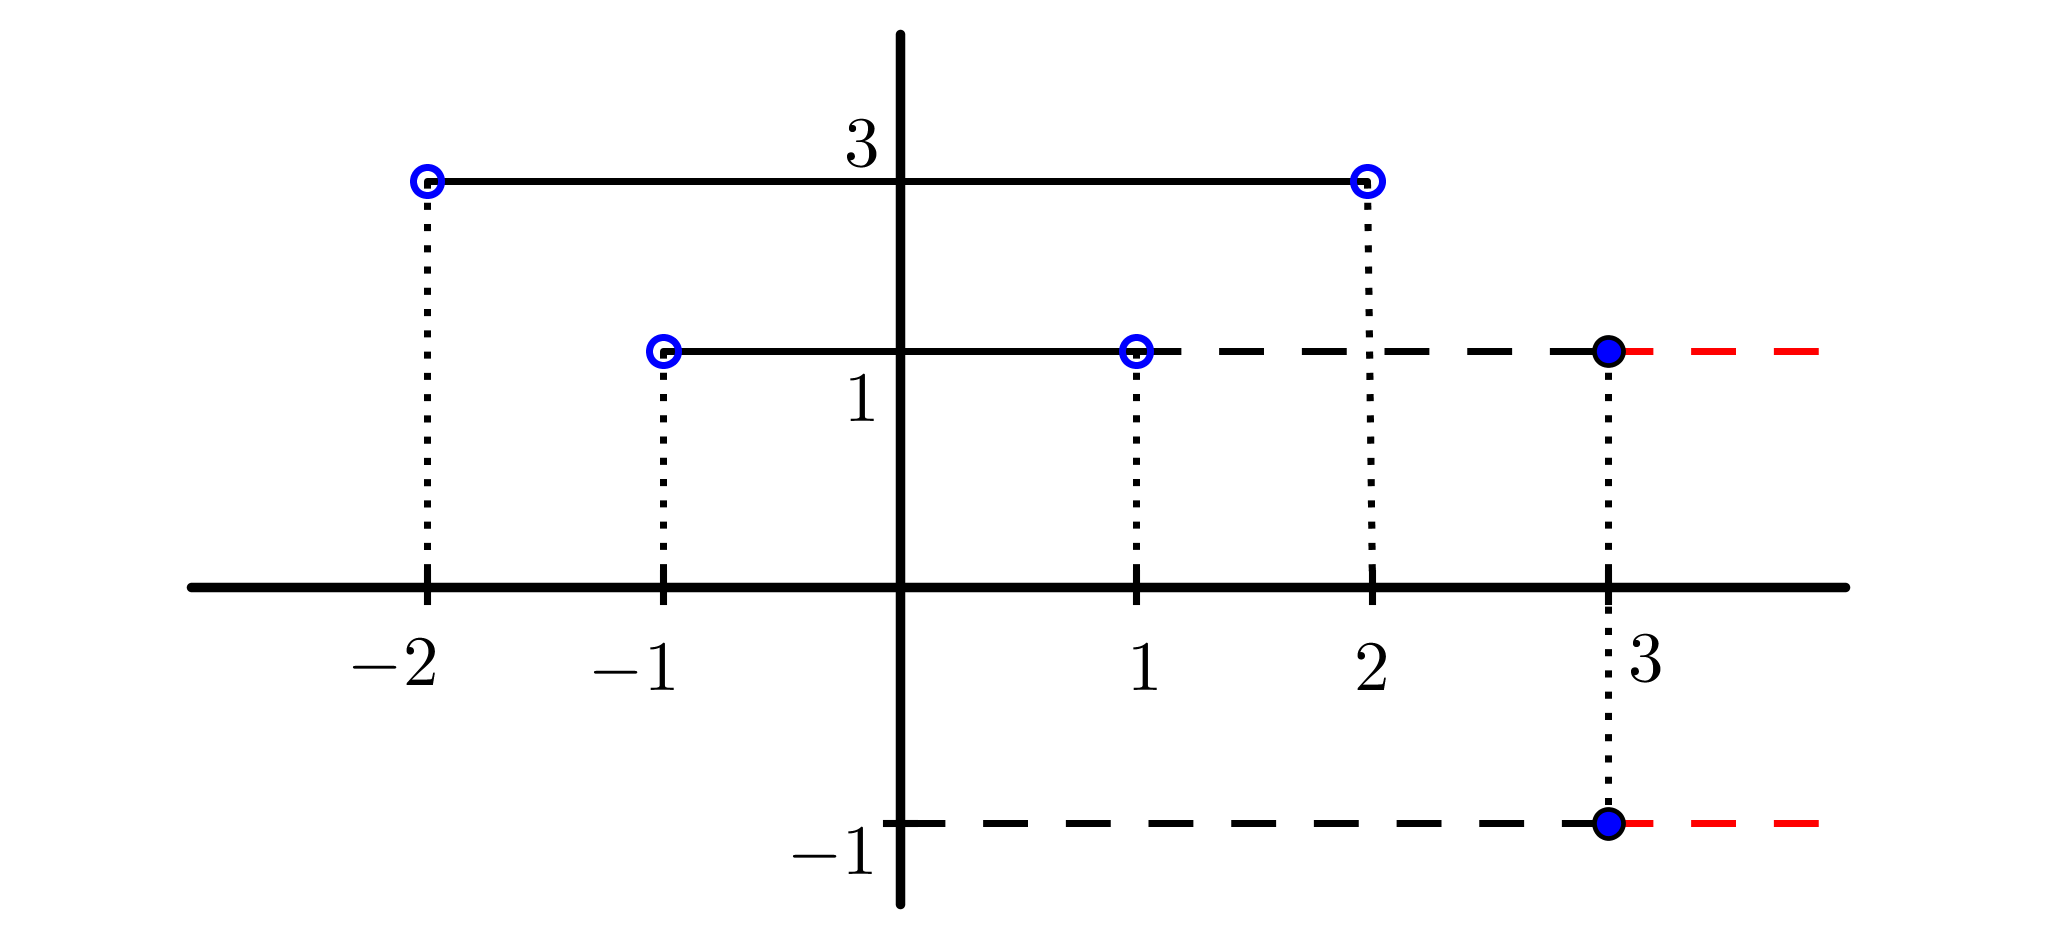
\includegraphics[width=.5\textwidth]{lebesgue-problem.png}
\caption{Problem \ref{094}}\label{fig094}
\end{figure}

\begin{align*}
f&=0\chi_{(-\infty,-2]}+3\chi_{[-2,-1]}+4\chi_{[-1,0]}+5\chi_{[0,1]}+4\chi_{[1,2]}+\chi_{[2,3]}+0\chi_{[3,\infty)}\\
 &=0\chi_{(-\infty,-2)\cup (3,\infty)}+\chi_{(2,3]}+3\chi_{[-2,-1)}+4\chi_{[-1,0)\cup (1,2]}+5\chi_{[0,1]}
\end{align*}
\end{proof}

\newpage
\section{General Measure Space}

\subsection{Definition}

\begin{defn}[\textbf{\color{blue}{Signed Measure}}]
A signed measure on $(X,\mathcal{M})$ means an extended real-valued set function
\[\nu: \mathcal{M}\to [-\infty,\infty]\qquad \mbox{such that}\]
\begin{description}
  \item[i)] $\nu$ assumes at most one of $+\infty$,$-\infty$.
  \item[ii)] $\nu(\emptyset)=0$.
  \item[iii)] For a countable collection $\{E_k\}_{k=1}^{\infty}$ of disjoint measurable sets
  \[\nu\biggl(\bigcup_{k=1}^{\infty}E_k\biggl)=\sum_{k=1}^{\infty}\nu(E_k)\]
  where $\sum_{k=1}^{\infty}\nu(E_k)$ converges absolutely if $\nu(\cup_{k=1}^{\infty}E_k)$ is finite.
\end{description}
\end{defn}

\begin{defn}[\textbf{\color{blue}{Positive Set}}]
A set $A$ is called positive with respect to a signed measure $\nu$ if $A$ is measurable and for every subset $E$ of $A$ we have $\nu(E)\geq 0$.
\end{defn}

\begin{defn}[\textbf{\color{blue}{Negative set}}]
A set $A$ is called negative with respect to a signed measure $\nu$ if $A$ is measurable and for every subset $E$ of $A$ we have $\nu(E)\leq 0$.
\end{defn}

\begin{defn}[\textbf{\color{blue}{Null set}}]
A set $A$ is said to be null if it is both positive and negative.
\end{defn}

\begin{defn}[\textbf{\color{blue}{Singular}}]
$\nu_1$ and $\nu_2$ defined on $\mathcal{M}$ are said to be singular $\nu_1\perp\nu_2$ if there are two disjoint measurable sets $A$ and $B$ such that $\nu_1(B)=\nu_2(A)=0$.
\end{defn}

\begin{defn}[\textbf{\color{blue}{Absolute Continuous Measure}}]
A measure $\nu$ on a measure space $(X,\mathcal{M})$ is said to be absolutely continuous the measure $\mu$ written $\nu\ll\mu$ if $\nu(A)=0$ for each $A$ with $\mu(A)=0$.
\end{defn}

\subsection{The $L^p$ Space}

\begin{defn}[\textbf{\color{blue}{Norm}}]
Define the norm of $f$ in $L^p$ by
\[\|f\|_p=\biggl[\int |f|^pd\mu\biggl]^{1/p}\]
\end{defn}
\begin{defn}[\textbf{\color{blue}{Conjugate Power}}]
The number $q$ is said to be a conjugate of $p$ if
\[\frac{1}{p}+\frac{1}{q}=1.\]
\end{defn}
\begin{thm}[\textbf{Young's Inequality}]
For $1<p<\infty$, $q$ the conjugate of $p$, and any two positive integer $a$ and $b$
\[ab\leq \frac{a^p}{p}+\frac{b^q}{q}\]
\end{thm}

\begin{proof}
Exercise
\end{proof}
\begin{thm}[\textbf{Holder's Inequality}]
Let $1<p<\infty$, $q$ a conjugate of $p$. If $f\in L^p(\mu)$ and $g\in L^q(\mu)$, then $fg\in L^1(\mu)$ and
\[\int |fg|d\mu \leq \biggl(\int|f|^pd\mu\biggl)^{1/p}\biggl(\int |g|^qd\mu\biggl)^{1/q}\]
\end{thm}

\begin{proof}
If $f=0$ a.e. or $g=0$ a.e., then the inequality holds. But if $f\neq 0$ and $g\neq 0$ a.e., then $\|f\|_p>0$ and $\|g\|_q>0$.\\
Now consider
\[F=\frac{|f|}{\|f\|_p},\qquad G=\frac{|g|}{\|g\|_q}\]
Notice that
\[\|F\|_p=1\qquad \mbox{and}\qquad \|G\|_q=1.\]
So it suffices to show
\[\int |fg|d\mu\leq 1\]
Now we use Young's inequality
\[FG\leq \frac{F^p}{p}+\frac{G^q}{q}\]
This implies
\[\int FG d\mu\leq \frac{\|F\|_p^p}{p}+\frac{\|G\|_q^q}{q}=\frac{1}{p}+\frac{1}{q}=1\]
Thus, the result follows.
\end{proof}

\begin{thm}[\textbf{Minkowski's Inequality}]
For $1\leq p<\infty$. Then for every pair of $f,g\in L^p(\mu)$ the following inequality holds
\[\|f+g\|_p\leq \|f\|_p+\|g\|_p\]
\end{thm}

\begin{proof}
If $p=1$, the inequality becomes trivial(triangle inequality). If $p>1$, consider
\begin{align*}
\int |f+g|^pd\mu &\leq \int (|f|+|g|)|f+g|^{p-1}d\mu\\
                 &=\int |f||f+g|^{p-1}d\mu+\int |g||f+g|^{p-1}d\mu\\
                 &\leq \|f\|_p\underbrace{\|(f+g)^{p-1}\|_q}_{\|f+g\|_p^{p-1}}+\|g\|_p\|(f+g)^{p-1}\|_q\tag{Holder}\\
                 &=\|f+g\|_p^{p-1}(\|f\|_p+\|g\|_p)
\end{align*}

\end{proof}

\subsection{Facts}

\begin{lem}
Let $X$ be a normed space. Then $X$ is complete if and only if every absolutely summable series is summable.
\end{lem}

\begin{proof}
Exercise
\end{proof}


\begin{thm}

\end{thm}

\begin{proof}
Exercise
\end{proof}

\newpage
\subsection{Exercise}
\begin{exer}\label{100}
Let $\{A_n\}$ be a countable collection of measurable sets, then
\[\mu\biggl(\bigcup_{k=1}^{\infty}A_k\biggl)=\lim_{n\to\infty} \mu\biggl(\bigcup_{k=1}^{\infty}A_k\biggl)\]
\end{exer}
\begin{exer}\label{100a}
Let $(X_{\alpha}, \mathcal{M}_{\alpha}, \mu_{\alpha})$ be a collection of measure spaces and suppose that the collection of sets $\{X_{\alpha}\}$ is disjoint. Then we can form a new measure space (called their union) $(X, \mathcal{B}, \mu)$ by letting $X =\bigcup X_{\alpha},$  define $ \mathcal{B}=\{B : \forall\alpha\ B\cap X_{\alpha}\in \mathcal{B}_{\alpha}\}$ and $\mu(B) =\sum \mu_{\alpha}(B\cap X_{\alpha}).$
\begin{description}
  \item[a)] Show that $\mathcal{M}$ is a $\sigma$-algebra.
  \item[b)] Show that $\mu$ is a measure.
  \item[c)] Show that $\mu$ is $\sigma$-finite if and only if all but a countable number of the measures $\mu_{\alpha}$ are zero and the remainder are $\sigma$-finite.
\end{description}
\end{exer}

\begin{exer}\label{100b}
Let $(X, \mathcal{M}, \mu)$ be a measure space. The symmetric difference, $E_1\Delta E_2$, of two subsets $E_1$ and $E_2$ of $X$ is defined by
\[ E_1\Delta E_2 = (E_1\backslash E_2)\cup (E_2\backslash E_1)\]
\begin{description}
  \item[a)] Show that if $E_1$ and $E_2$ are measurable and $\mu(E_1\Delta E_2) = 0$, then $\mu(E_1)=\mu(E_2)$.
  \item[b)] Show that if $\mu$ is complete, $E_1\in \mathcal{M}$ and $E_2\backslash E_1\in \mathcal{M}$, then $E_2\in \mathcal{M}$ if $\mu(E_1\Delta E_2)=0$.
\end{description}
\end{exer}

\begin{exer}[\textbf{Hardy's Inequality}]\label{101}
Suppose that $f\geq 0$ on $(0,\infty)$, $f\in L^{p}(0,\infty)$ and
  \[F(x)=\frac{1}{x}\int_0^x f(t)dt\]
  Prove that for $1<p<\infty$
  \[\int_{0}^{\infty}(F(x))^p dx\leq \biggl(\frac{p}{p-1}\biggl)^p\int_0^{\infty}(f(t))^pdt\]
  Hint: Write $xF(x)=\int_{0}^{x}f(t)t^{a}\cdot t^{-a}dt$ and use Holder's inequality.
\end{exer}

\begin{exer}\label{102}
Let $f,\{f_k\}\in L^p$ where $1\leq p<\infty$. Show that if $\|f-f_k\|_p\to 0$, then $\|f_k\|_p\to\|f\|_p$. Conversely if $f_k\to f$ a.e and $\|f_k\|_p\to\|f\|_p$, show that $\|f-f_k\|_p \to 0$.
\end{exer}

\begin{exer}\label{103}

\end{exer}

\newpage
\subsection*{Solution}
\begin{proof}[Solution (\ref{100})]
Let $\{A_n\}$ be a collection of measurable sets. Let $B_1 = A_1$ and $B_k = A_k \ \cup_{k=1}^{n-1}A_n$ for $k>1$.
Then $\{B_n\}$ is a collection of pairwise disjoint measurable sets such that $\cup A_n =\cup B_n$. Now
\[\mu(\cup A_k) =\mu(\cup B_k) =\sum \mu(B_k) = \lim_n \sum_{k=1}^n\mu(B_k)=\lim_n \mu(\cup_{k=1}^n B_k)=\lim_n \mu(\cup_{k=1}^n A_k).\]
\end{proof}

\begin{proof}[Solution (\ref{100a})]
Exercise.
\end{proof}

\begin{proof}[Solution (\ref{100b})]
Exercise.
\end{proof}

\begin{proof}[Solution (\ref{101})]
We start with
  \[\int_{0}^{\infty} F(x)^pdx =\int_{0}^{\infty}\frac{1}{x^p}\biggl(\int_0^x f(t)dt\biggl)^p dx.\]
  Now use the hint, and write
  \[\int_0^x f(t)dt =\int_0^x f(t)t^at^{-a}dt\]
  where $0 < a < \frac{1}{q}= 1-\frac{1}{p}$. We apply Holder’s Inequality to this expression to get that
  \[\int_0^x f(t)dt \leq \biggl(\int_0^x f(t)^pt^{ap}dt\biggl)^{\frac{1}{p}}\biggl(\int_0^x t^{-aq}dt\biggl)^{\frac{1}{q}}=\frac{x^{\frac{1}{q}-a}}{(1-aq)^{\frac{1}{q}}}\biggl(\int_0^x f(t)^pt^{ap}dt\biggl)^{\frac{1}{p}}.\]
  Using this estimate we find
  \begin{align*}
  \int_0^{\infty} F(x)^p dx &= \int_0^{\infty} \frac{1}{x^p}\biggl(\int_0^x f(t)dt\biggl)^p dx\\
                             &\leq \frac{1}{(1-aq)^{\frac{p}{q}}}\int_0^{\infty} x^{\frac{p}{q}-pa-p}\biggl(\int_0^x f(t)^pt^{ap}dt\biggl) dx\\
                             &=\frac{1}{(1-aq)^{\frac{p}{q}}}\int_0^{\infty} f(t)^pt^{ap}\biggl(\int_t^{\infty}x^{\frac{p}{q}-pa-p}dx\biggl)dt.
  \end{align*}
  Now note that
  \[\int_t^{\infty} x^{\frac{p}{q}-pa-p}dx =\int_t^{\infty} x^{-1-pa}dx = t^{-pa}\frac{1}{ap},\]
  and so we have
  \[\int_0^{\infty} F(x)^pdx\leq \frac{1}{ap(1-aq)^{\frac{p}{q}}}\int_0^{\infty} f(t)^pdt.\]
  Choose now $a =\frac{1}{p+q}$, which is found by solving a minimization problem, and then simple algebra gives
  \[\frac{1}{ap(1-aq)^{\frac{p}{q}}}= \biggl(\frac{p}{p-1}\biggl).\]
\end{proof}
\begin{proof}[Solution (\ref{102})]
By Minkowski's inequality, $\biggl |\|f\|_p-\|f_k\|_p\biggl |\leq \|f-f_k\|_p$, so $\|f-f_k\|_p\to 0$ implies $\|f_k\|_p\to \|f\|_p$. (If $p < 1$, we have $\biggl | \|f\|_p-\|f_k\|_p\biggl|\leq c\|f-f_k\|_p$ for some $c > 1$, so the argument still holds.) For the converse, since $p\geq 1$, we have
  \[ |f-f_k|^p \leq 2^{p-1} (|f|^p + |f_k|^p),\]
  so by Fatou’s lemma and the fact that $f_k\to f$ a.e., we have
  \begin{align*}
  \int 2^p |f|^p &=\int \liminf_k 2^{p-1} (|f|^p + |f_k|^p)-|f-f_k|^p\\
                 &\leq \liminf_k\int 2^{p-1} (|f|^p + |f_k|^p) + \liminf_k -\int|f- f_k|^p\\
                 &= \lim_k\int 2^{p-1} (|f|^p + |f_k|^p)-\limsup_k\int|f-f_k|^p\\
                 &= \int 2^p |f|^p -\limsup_k\int|f-f_k|^p ,
  \end{align*}
  where the last equality follows by the dominated convergence theorem since $|f|^p$ and $|f_k|^p$ are in $L^1$. Thus, $\limsup_k \int|f-f_k|^p\leq 0$, so $\|f-f_k\|_p\to 0$.
\end{proof}
\begin{proof}[Solution (\ref{103})]
Exercise.
\end{proof}

\newpage

\begin{thebibliography}{9}

\bibitem{July}
Stephen Abbott, 2001,
Understanding Analysis. Undergraduate Text in Mathematics, SpringerVerlag, New York.

\bibitem{Maybe}
[Iain T. Adamson] ~
A General Topology Workbook, published by Birkh$\ddot{a}$user Boston in 1996.

\bibitem{Jun}
[Tom Apostol]~
Mathematical Analysis, Second Edition, Addison-Wesley, Reading, MA,
1974.

\bibitem{May}
[Robert Bartle \& Donald R.] ~
Introduction to Real Analysis, third edition, John Wiley \& Sons, Inc. 2000.

\bibitem{Sep}
[Seymour Lipschutz]~
Schaum's Outline of Theory and Problems of Genereal Topology, McGraw-Hill, New York, 1965.

\bibitem{notamsshort}
[Hans Sagan]  ~
Advanced Calculus of Real-Valued Functions of  a Real Variable and Vecter-Valued Functions of a Vector Variable.

\bibitem{notshort}
[Y. Sagher]  ~
Counting the rationals. American Mathematical Monthly 96, 823.

\bibitem{short}
[Royden \& Fitzpatrick]  ~
Real Analysis,  the Macmillan Company, New York , 1963.

\bibitem{amsshort}
[Walter Rudin]  ~
Principles of Mathematical Analysis. International Series in Pure and Applied
Mathematics, McGraw-Hill, New York, 1964.

\end{thebibliography}
\end{document}
